% Created 2026-04-23 Thu 12:09
% Intended LaTeX compiler: lualatex
\DocumentMetadata{lang = en-US,pdfversion = 2.0,pdfstandard = ua-2,tagging = on,tagging-setup = {math/setup=mathml-SE},}
\documentclass[11pt]{article}
\usepackage{amsmath}
\usepackage{fontspec}
\usepackage{graphicx}
\usepackage{longtable}
\usepackage{wrapfig}
\usepackage{rotating}
\usepackage[normalem]{ulem}
\usepackage{capt-of}
\usepackage{hyperref}
\usepackage[margin=1in]{geometry}
\usepackage{fontspec}
\usepackage{verbatim, multicol, tabularx,}
\usepackage{amsmath, amsthm, amssymb, stmaryrd, latexsym, bm, listings, qtree}
\usepackage{framed}
\usepackage{xcolor,colortbl}
\usepackage{media9}
\usepackage[export]{adjustbox}
\usepackage{algorithm}
\usepackage[noend]{algpseudocode}
\usepackage{tikz,pgfplots}
\usetikzlibrary{shapes.geometric}
\let\oldquote=\quote
\let\endoldquote=\endquote
\colorlet{shadecolor}{cyan!15}
\renewenvironment{quote}{\begin{shaded*}\begin{oldquote}}{\end{oldquote}\end{shaded*}}
% From https://tex.stackexchange.com/questions/7032/good-way-to-make-textcircled-numbers
\newcommand*\circled[1]{\tikz[baseline=(char.base)]{\node[shape=circle,draw,inner sep=2pt] (char) {#1};}}
\DeclareMathOperator*{\argmin}{arg\!min}
\DeclareMathOperator*{\argmax}{arg\!max}
\lstset{frame=tb, aboveskip=1mm, belowskip=0mm, showstringspaces=false, columns=flexible, basicstyle={\scriptsize\ttfamily}, numbers=left, frame=single, breaklines=true, breakatwhitespace=true}
\hypersetup{colorlinks=true,urlcolor=blue}
\usepackage{tagpdf}
\tagpdfsetup{activate-all}
\tagpdfsetup{math/alt/use}
\usepackage{polyglossia}
\setdefaultlanguage[variant=en-US]{english}
\author{Christopher Simpkins}
\date{Kennesaw State University}
\title{Artificial Intelligence\\\medskip
\large Problem Solving}
\hypersetup{
 pdfauthor={Christopher Simpkins},
 pdftitle={Artificial Intelligence},
 pdfkeywords={},
 pdfsubject={Artificial Intelligence Problem Solving},
 pdfcreator={Emacs 30.2 (Org mode 9.7.11)}, 
 pdflang={English}}
\begin{document}

\maketitle
\section{Planning Agents}
\label{sec:org1a90ea7}

\begin{itemize}
\item Problem Solving Agents
\item Search Problems and Solutions
\item Search Algorithms
\item Elements of Search Algorithm Implementations
\item Uninformed Search
\end{itemize}
\section{Problem-Solving Agents}
\label{sec:org27e93f3}


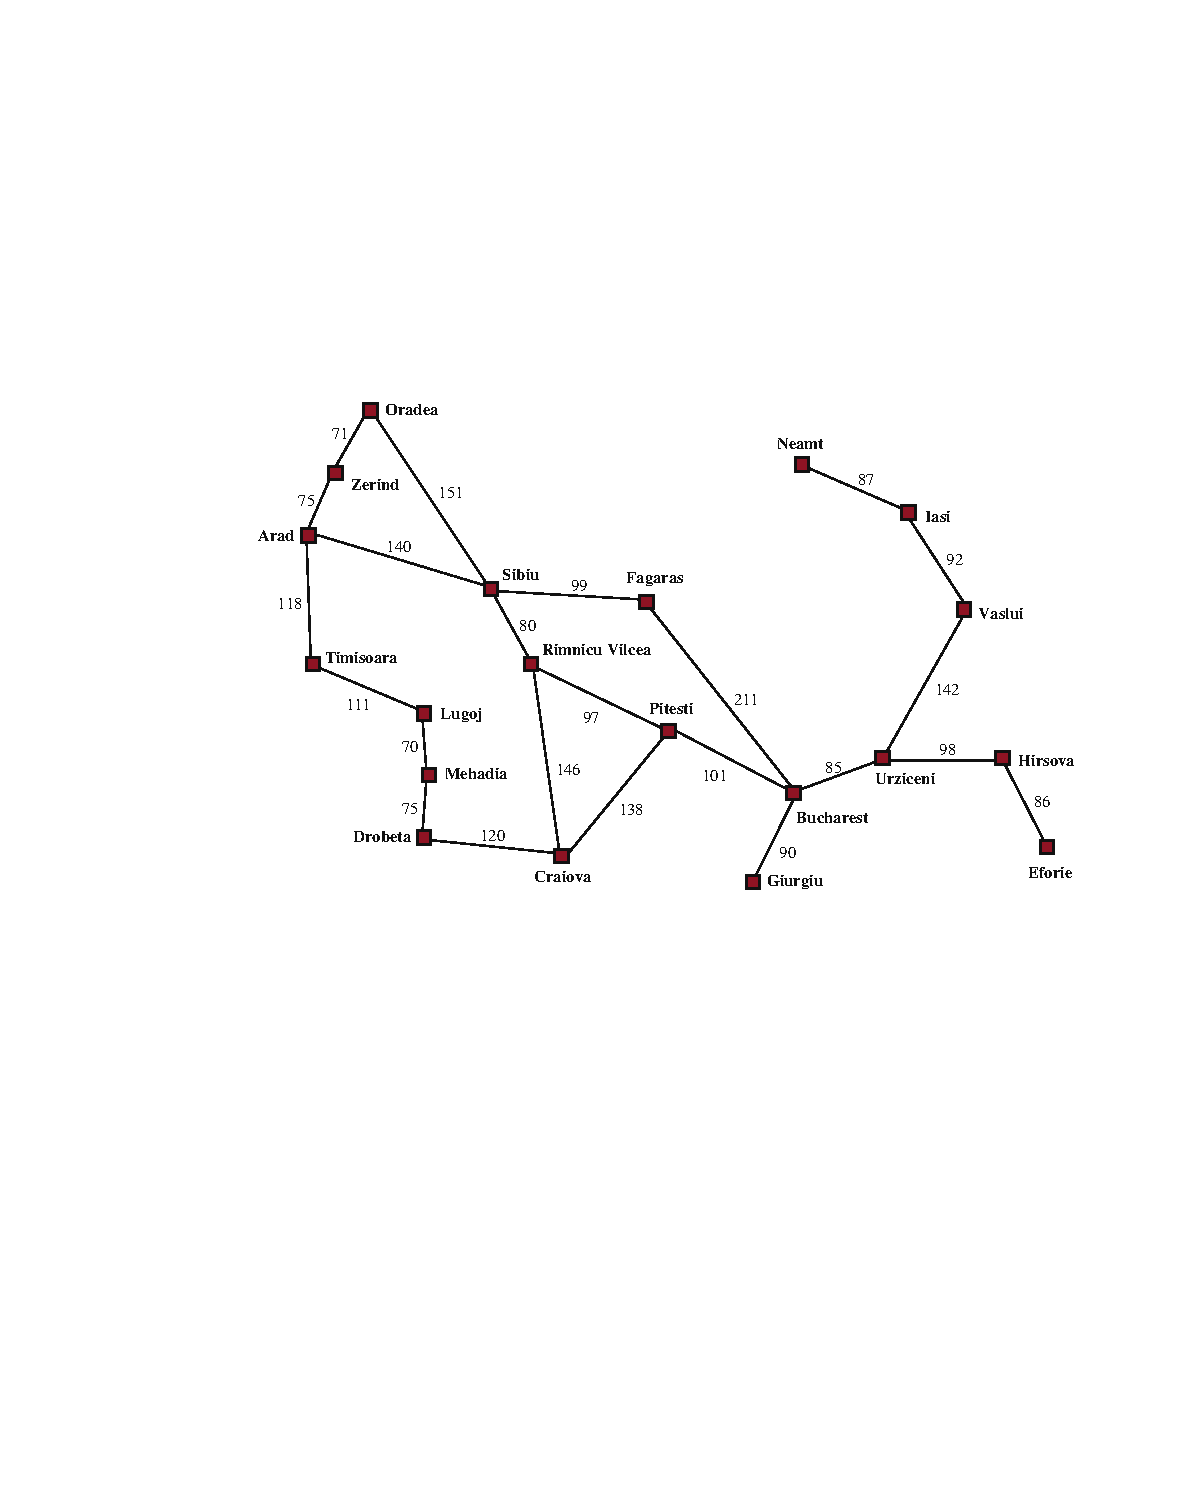
\includegraphics[alt={aima fig 03_01 romania},height=2.4in]{aima-fig-03_01-romania.pdf}


\begin{itemize}
\item In this lesson we consider a \textbf{state} to be our location in one of these cities.
\item A \textbf{goal} is a state in which we are located in a particular city.
\end{itemize}

This is the essence of problem solving: transforming a current state into a goal state.  The first family of algorithms we'll study for problem solving are \textbf{search} algorithms.
\section{Problem Solving Process}
\label{sec:org82b029d}

To solve a problem, we

\begin{itemize}
\item Formulate a \textbf{goal}, e.g., "reach Bucharest"
\item Formulate the \textbf{problem} as a set of states and actions that move us from one state to another.

\begin{itemize}
\item Problem is a \textbf{model} -- an \textbf{abstract} mathematical description.
\item Abstraction is essence and ignorance.
\item Key skill in problem formulation is finding the right \textbf{level of abstraction}.
\end{itemize}

\item \textbf{Search} the possible sequences of action in our problem model that transforms our state from the current state to the goal state.  A sequence of actions that gets us to the goal state is called a \textbf{solution}.  May be many; pick one.
\item \textbf{Execute} the actions in the solution.
\end{itemize}
\section{Open-Loop vs. Closed-Loop Control}
\label{sec:org62f4cef}

\begin{itemize}
\item In an \textbf{open-loop} system the agent gets no feedback, i.e., sensor input, after executing an action.

\begin{itemize}
\item If the agent's model is perfect and actions are deterministic, then the agent can operate in an open-loop fashion, simply executing the actions in the solution one after the other.
\end{itemize}

\item In a \textbf{closed-loop} system gets sensory feedback after every action, so it can check whether the action had the expected effect.

\begin{itemize}
\item If the environment is partially observable or actions are nondeterministic, closed-loop control is necessary.
\item Say the agent executes to \texttt{ToSibiu} action but ends up in \texttt{Zerind}.  Closed-loop feedback will alert the agent to this fact so it can re-plan.
\end{itemize}
\end{itemize}
\section{Search Problems}
\label{sec:org78938fb}

A search problem consists of:

\begin{itemize}
\item A set of \textbf{states}, which we call a \textbf{state space}.
\item \textbf{Initial state}
\item A set of \textbf{goal states}.

\begin{itemize}
\item Typically use an `IS-GOAL(s)` predicate function to identify goal states.
\end{itemize}

\item Sets of \textbf{actions} available in each state, `ACTION(s)`

\begin{itemize}
\item `ACTION(Arad) = \{ToSibiu, ToTimisoara, ToZerind\}`
\end{itemize}

\item A \textbf{transition model}, `RESULT(s, a)`

\begin{itemize}
\item `RESULT(Arad, ToZerind) = Zerind`
\end{itemize}

\item An \textbf{action cost function}, `ACTION-COST(s, a, s')` or \(c(s, a, s')\) which returns the cost of executing action \(a\) in state \(s\) and reaching state \(s'\).
\end{itemize}
\section{Solution}
\label{sec:org20c4665}

\begin{itemize}
\item A solution is a path from the start state to the a goal state.
\item An optimal solution is a solution with lowest cost among all solutions.
\end{itemize}


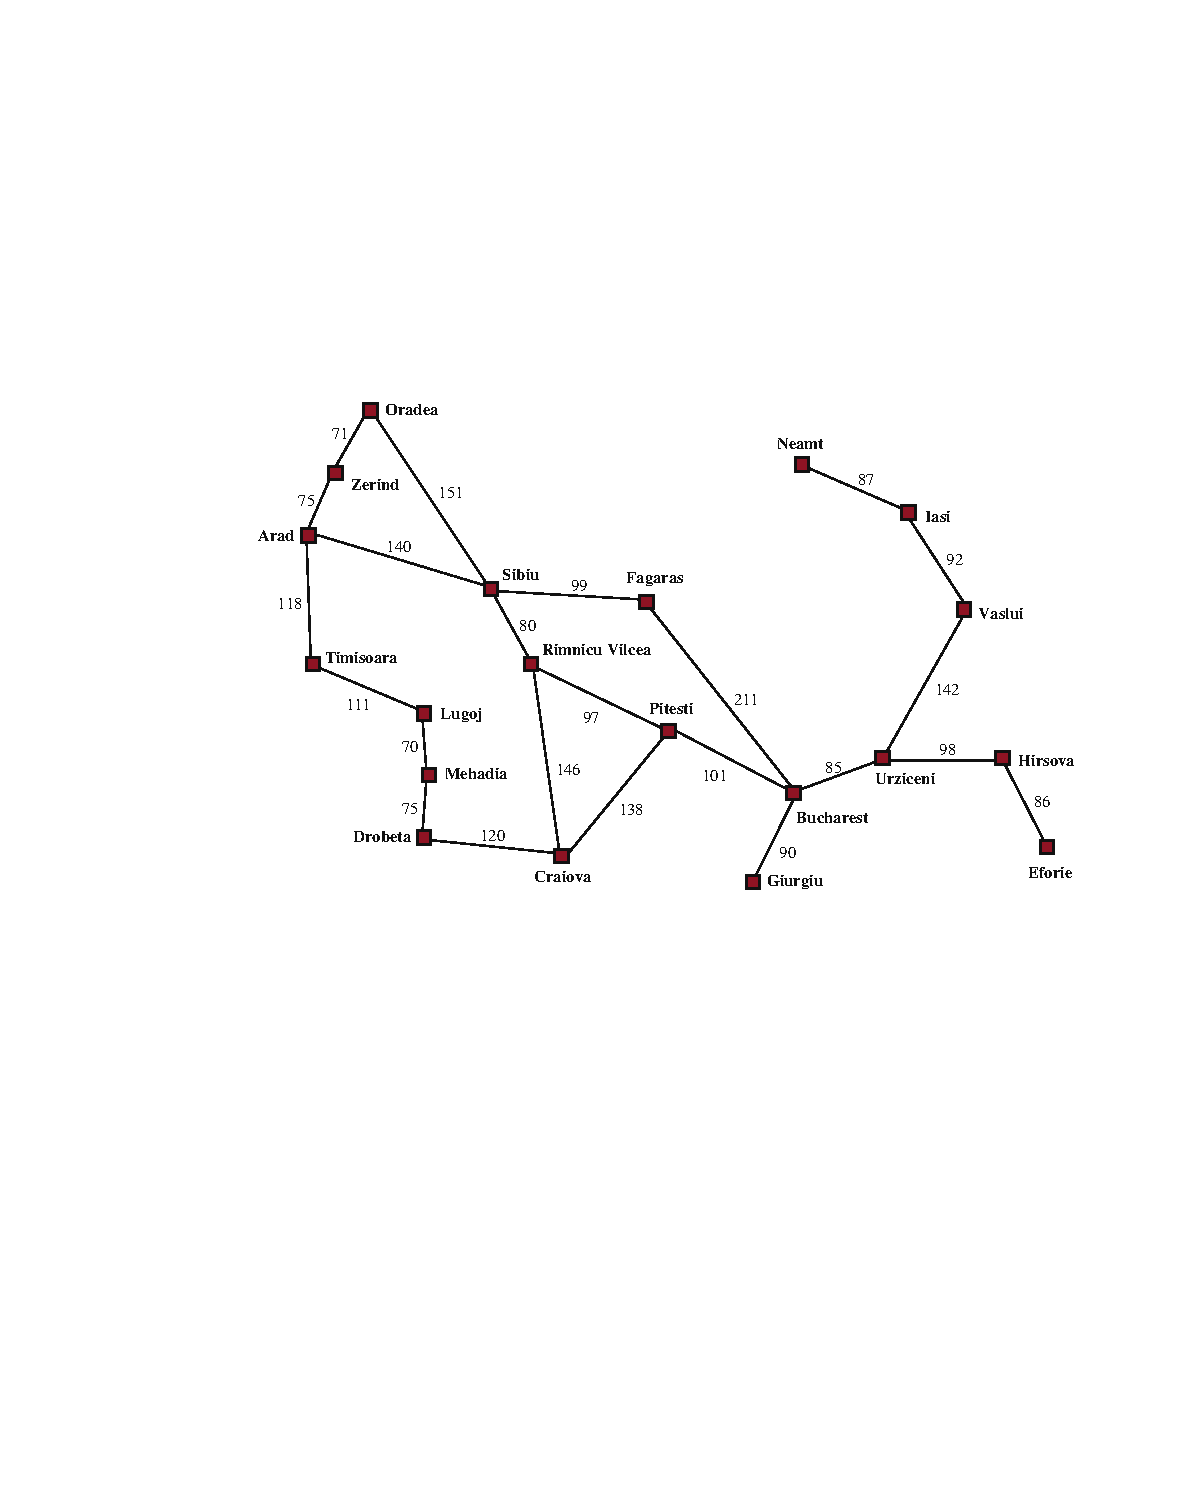
\includegraphics[alt={aima fig 03_01 romania},height=2.4in]{aima-fig-03_01-romania.pdf}

\begin{itemize}
\item How many paths are there from \texttt{Arad} to \texttt{Bucharest}?
\item What is/are the solutions to the `Arad-to-Bucharest` problem (assume perfect information -- fully observable, known dynamics, and deterministic actions)?
\end{itemize}
\section{Example Problems}
\label{sec:orgad8c030}

\begin{itemize}
\item \textbf{Standardized problems} use idealized environments designed to illustrate or exercise various problem-solving methods.  See, for example, \href{https://gymnasium.farama.org/}{Gymnasium}.

\begin{itemize}
\item A \textbf{grid world} is an standardized environment whose states are organized as a grid, and whose actions include moving between adjacent grids.
\end{itemize}
\end{itemize}


\begin{itemize}
\item \textbf{Real-world problems} are formulated for specific real-world tasks, like the problem specification used for Rhoombas.
\end{itemize}

Here's a standardized environment for the vacuum cleaner agent, formulated as a grid world:


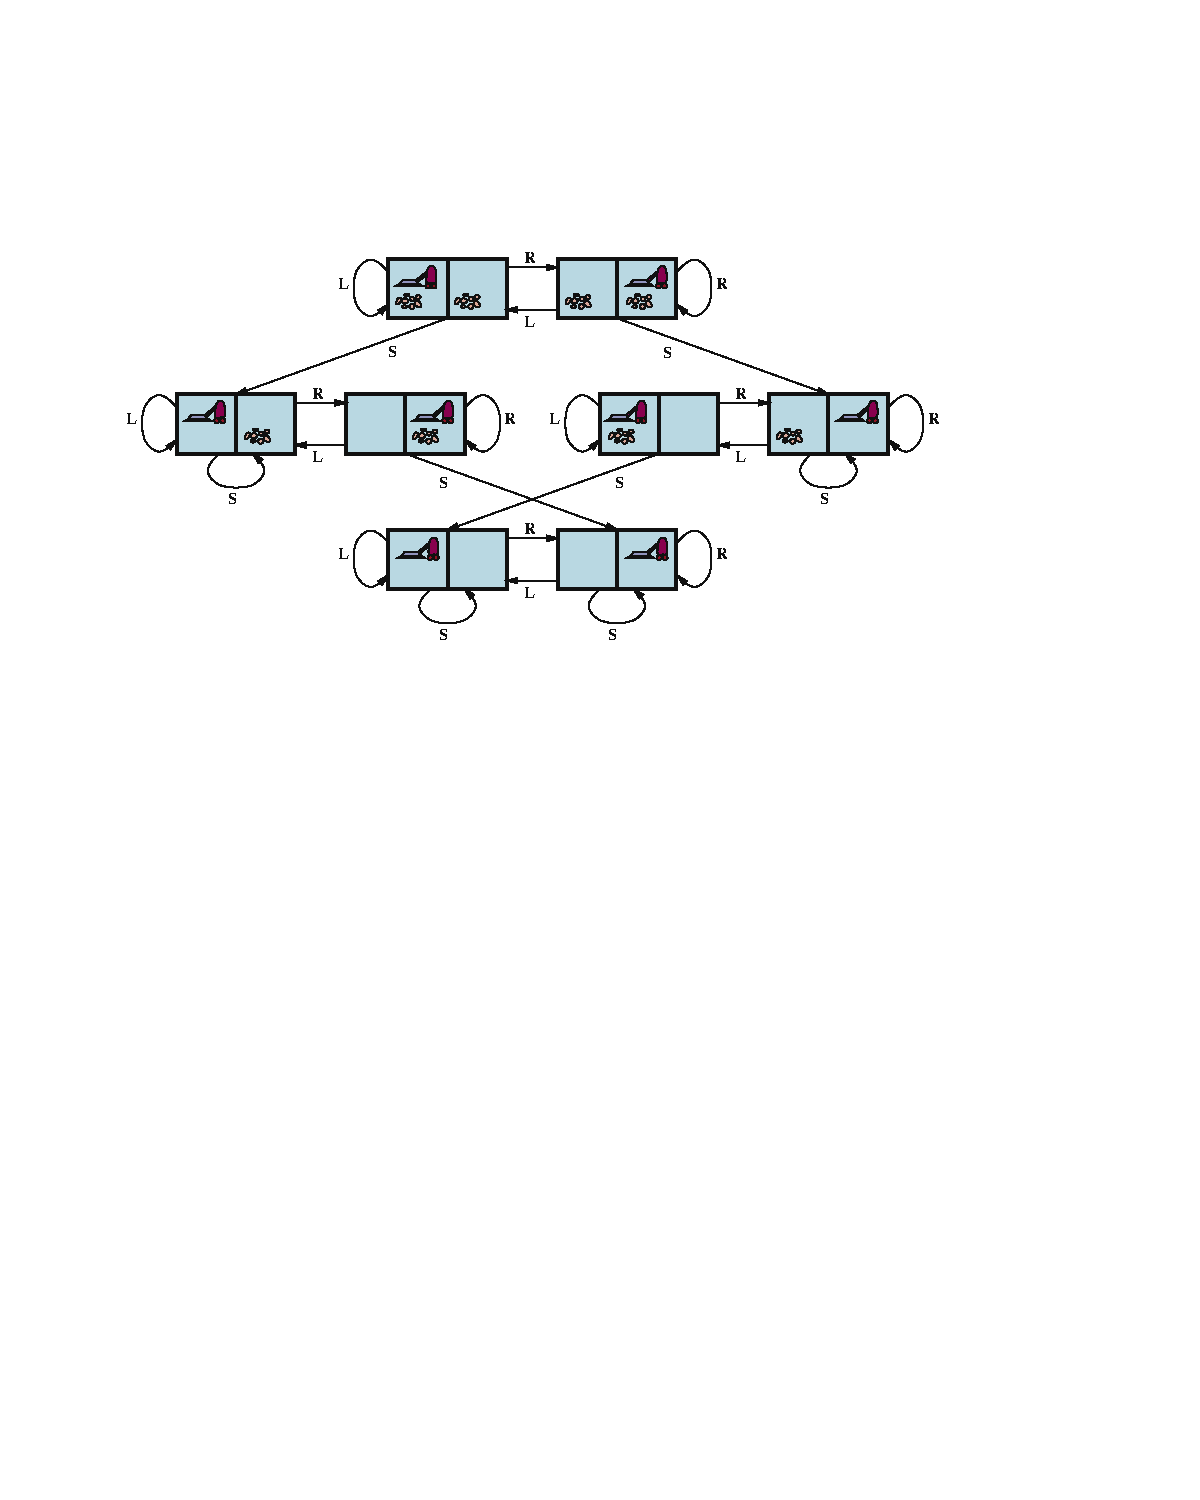
\includegraphics[alt={aima fig 03_02 vacuum state space graph},height=2.0in]{aima-fig-03_02-vacuum-state-space-graph.pdf}
\section{Vacuum Cleaner Grid World}
\label{sec:orgb52b96c}


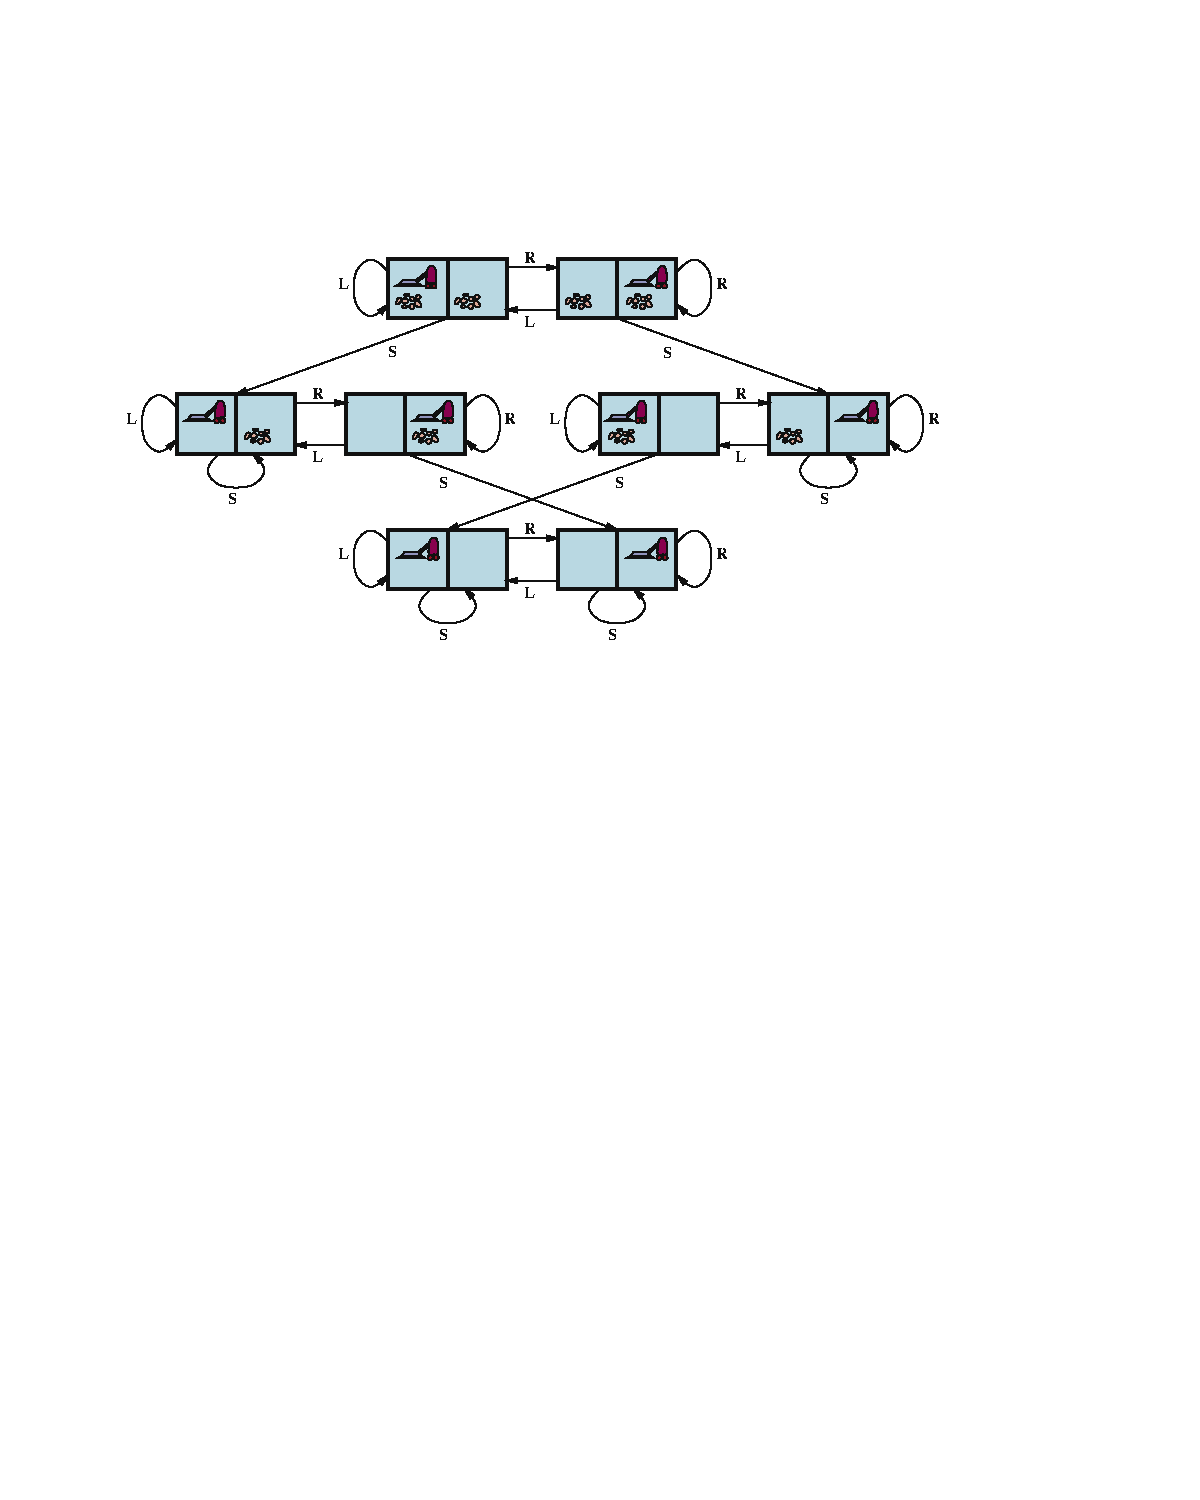
\includegraphics[alt={aima fig 03_02 vacuum state space graph},height=1.6in]{aima-fig-03_02-vacuum-state-space-graph.pdf}


\begin{itemize}
\item \textbf{States} include both the agent's location, and characteristics of the environment.  For the vacuum world, that's \(2 \cdot 2^2 = 8\) states.
\item \textbf{Initial state} is an arbitrary choice of the possible states.  Sometimes this choice is important.
\item \textbf{Actions} for this vacuum world are are \texttt{L}, \texttt{R}, and \texttt{Suck}.

\begin{itemize}
\item For 2D grids we can choose between

\begin{itemize}
\item \textbf{absolute} movement, like \texttt{Up} and \texttt{Right}, a.k.a., cardinal directions, or
\item \textbf{egocentric} movement, like \texttt{TurnRight}, \texttt{MoveForward}.  How does this affect the state description?
\end{itemize}
\end{itemize}

\item \textbf{Goal states} are those in which every location is clean.
\item \textbf{Action cost} (path cost) is 1.
\end{itemize}
\section{Route Finding}
\label{sec:org4377b0f}

\begin{itemize}
\item \textbf{States}: a location (e.g., an airport) and the time.

\begin{itemize}
\item If action cost (e.g., a flight segment) depends on previous segments, fares, etc., the state must include these details.
\end{itemize}

\item \textbf{Initial state}: The user’s home airport.
\item \textbf{Actions}: Take any flight from the current location, in any seat class, leaving after the current time, or for connecting flights, after sufficient in-airport transfer time.
\item \textbf{Transition model}: The state resulting from taking a flight will have the flight’s destination as the new location and the flight’s arrival time as the new time.

\begin{itemize}
\item Example \(T(s, a, s')\): `T(S(ATL, 10:00), A(DL875), S(LGA, 12:00))` (DL875 has a flight time of 2 hours).
\end{itemize}

\item \textbf{Goal state}: A destination city. Sometimes the goal can be more complex, such as arrive at the destination on a nonstop flight.  (Remember, a solution is a path, i.e., sequence of actions.)
\item \textbf{Action cost}: A combination of monetary cost, waiting time, flight time, customs and immigration procedures, seat quality, time of day, type of airplane, frequent-flyer reward points, and so on.
\end{itemize}
\section{Real-World Problems}
\label{sec:org8de28ca}

\begin{itemize}
\item \textbf{Touring problems}
\item \textbf{VLSI layout} -- minimize area, minimize circuit delays, minimize stray capacitances, and maximize manufacturing yield

\begin{itemize}
\item Cell layout -- place cells on chip so they don't overlap and have room for connections
\item Channel routing -- find routes for each wire between cells
\end{itemize}

\item \textbf{Robot navigation}
\item \textbf{Automatic assembly sequencing} -- standard practice in manufacturing since the 1970s.

\begin{itemize}
\item Solving some automatic assembly problems could earn you a \href{https://deepmind.google/science/alphafold/}{Nobel Prize!}
\end{itemize}
\end{itemize}
\section{Search Algorithms}
\label{sec:org614fde9}

A \textbf{search algorithm} takes a search problem as input and returns a solution, or an indication of failure.

\begin{itemize}
\item In general, the states and actions of a problem create a state space graph.
\item Here we consider algorithms that superimpose a \textbf{search tree} over the state-space graph.
\item \textbf{Nodes} correspond to states, \textbf{edges} correspond to actions
\end{itemize}

Don't confuse state space with search tree.

\begin{itemize}
\item State space is set of states, and actions that cause transitions between states.
\item Search tree describes paths between these states, reaching towards the goal(s).

\begin{itemize}
\item May be many nodes for a given state, but each path from root to node is unique.
\end{itemize}
\end{itemize}

Here is a search tree being imposed on the Romania state space graph by a search algorithm.


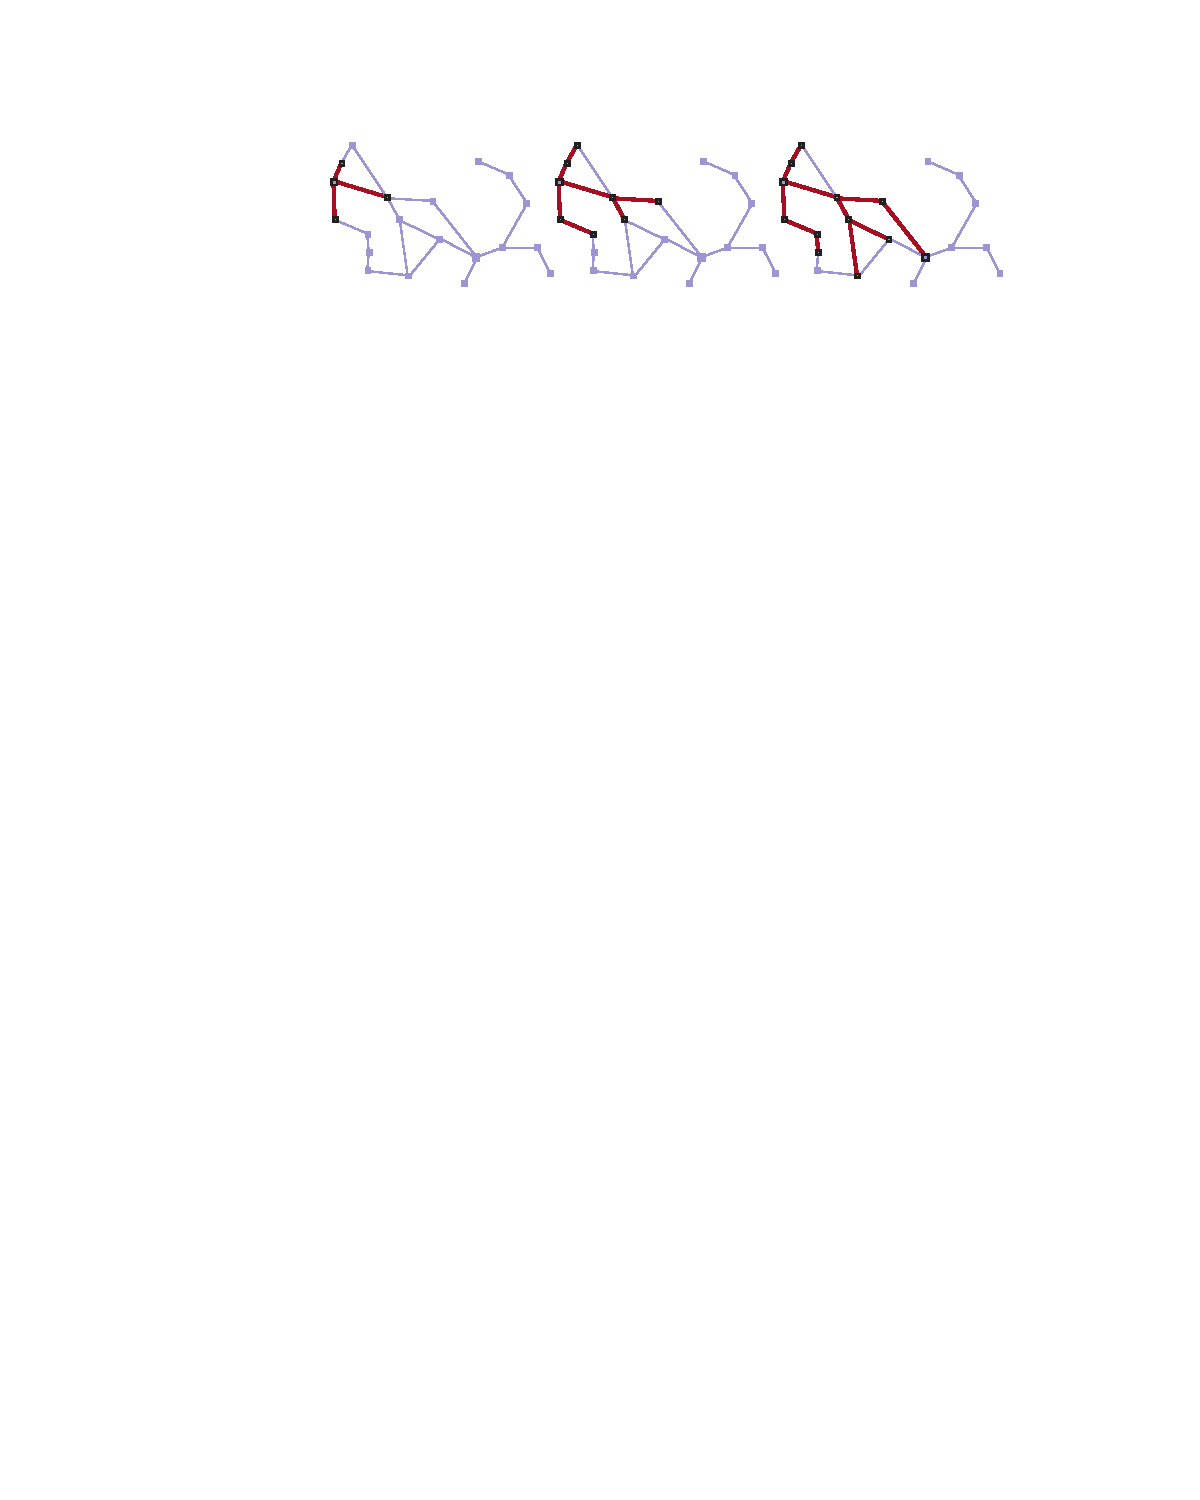
\includegraphics[alt={aima fig 03_05 search tree expansion},width=0.75\linewidth]{aima-fig-03_05-search-tree-expansion.pdf}
\section{Elements of Search Algorithms}
\label{sec:org903a791}

Essence of search:

\begin{itemize}
\item Choose a child node to consider next.  "Who's first?"
\item Put aside other nodes for later. "Who's next?"
\end{itemize}

Root node is initial state.  At each node we can \textbf{expand} the node, which grows the tree, by taking actions (adding edges) that lead to successor states (generate successor/child nodes).  Search algorithms must keep track of:

\begin{itemize}
\item \textbf{Expanded} nodes.  We test expanded nodes before dealing with frontier.
\item \textbf{Frontier} nodes, which are generated but not yet expanded.

\begin{itemize}
\item \textbf{Reached} = \textbf{Expanded} + \textbf{Frontier}
\end{itemize}
\end{itemize}
\section{Search Progression}
\label{sec:org6ed054f}


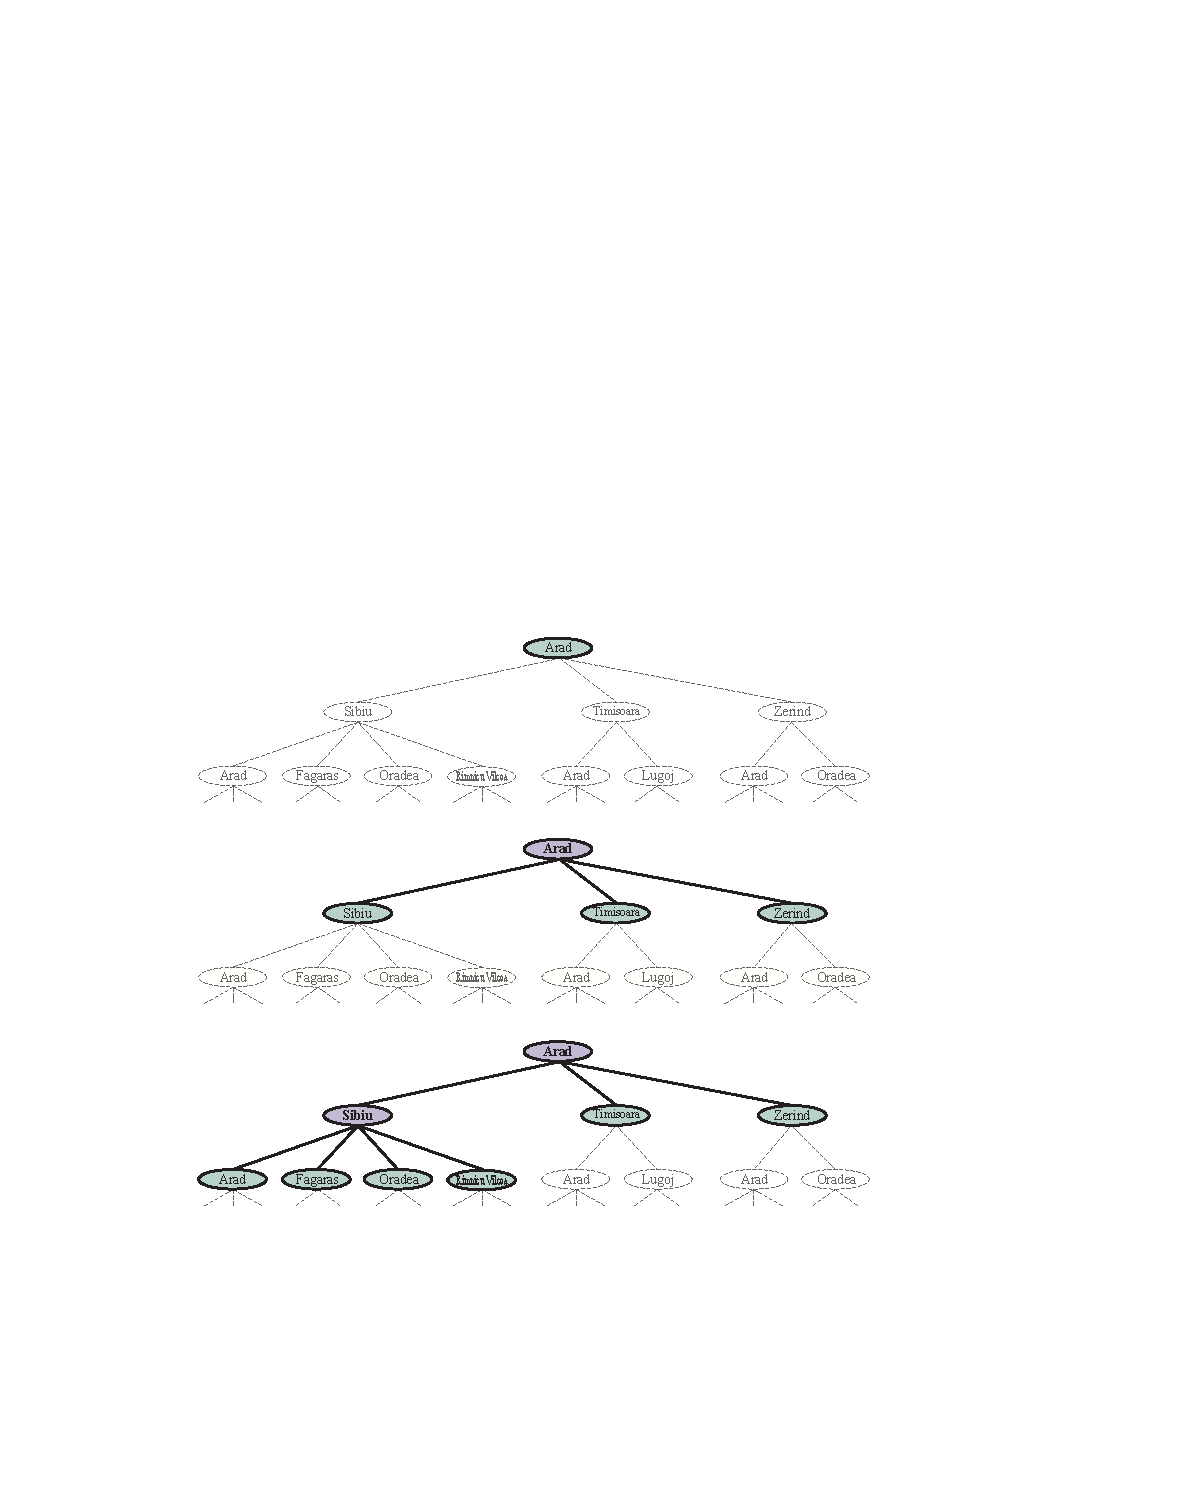
\includegraphics[alt={aima fig 03_04 arad bucharest partial trees},height=3.0in]{aima-fig-03_04-arad-bucharest-partial-trees.pdf}


\begin{itemize}
\item \textbf{Expanded} nodes are lavender with bold letters.
\item \textbf{Frontier} nodes are green with normal weight font.
\item Nodes in dashed-line ovals are candidates for expansion.
\end{itemize}
\section{Separation Property of Graph Search}
\label{sec:org1c1d30f}

The \textbf{frontier} separates the interior region of expanded nodes from the exterior region of unexpanded nodes.


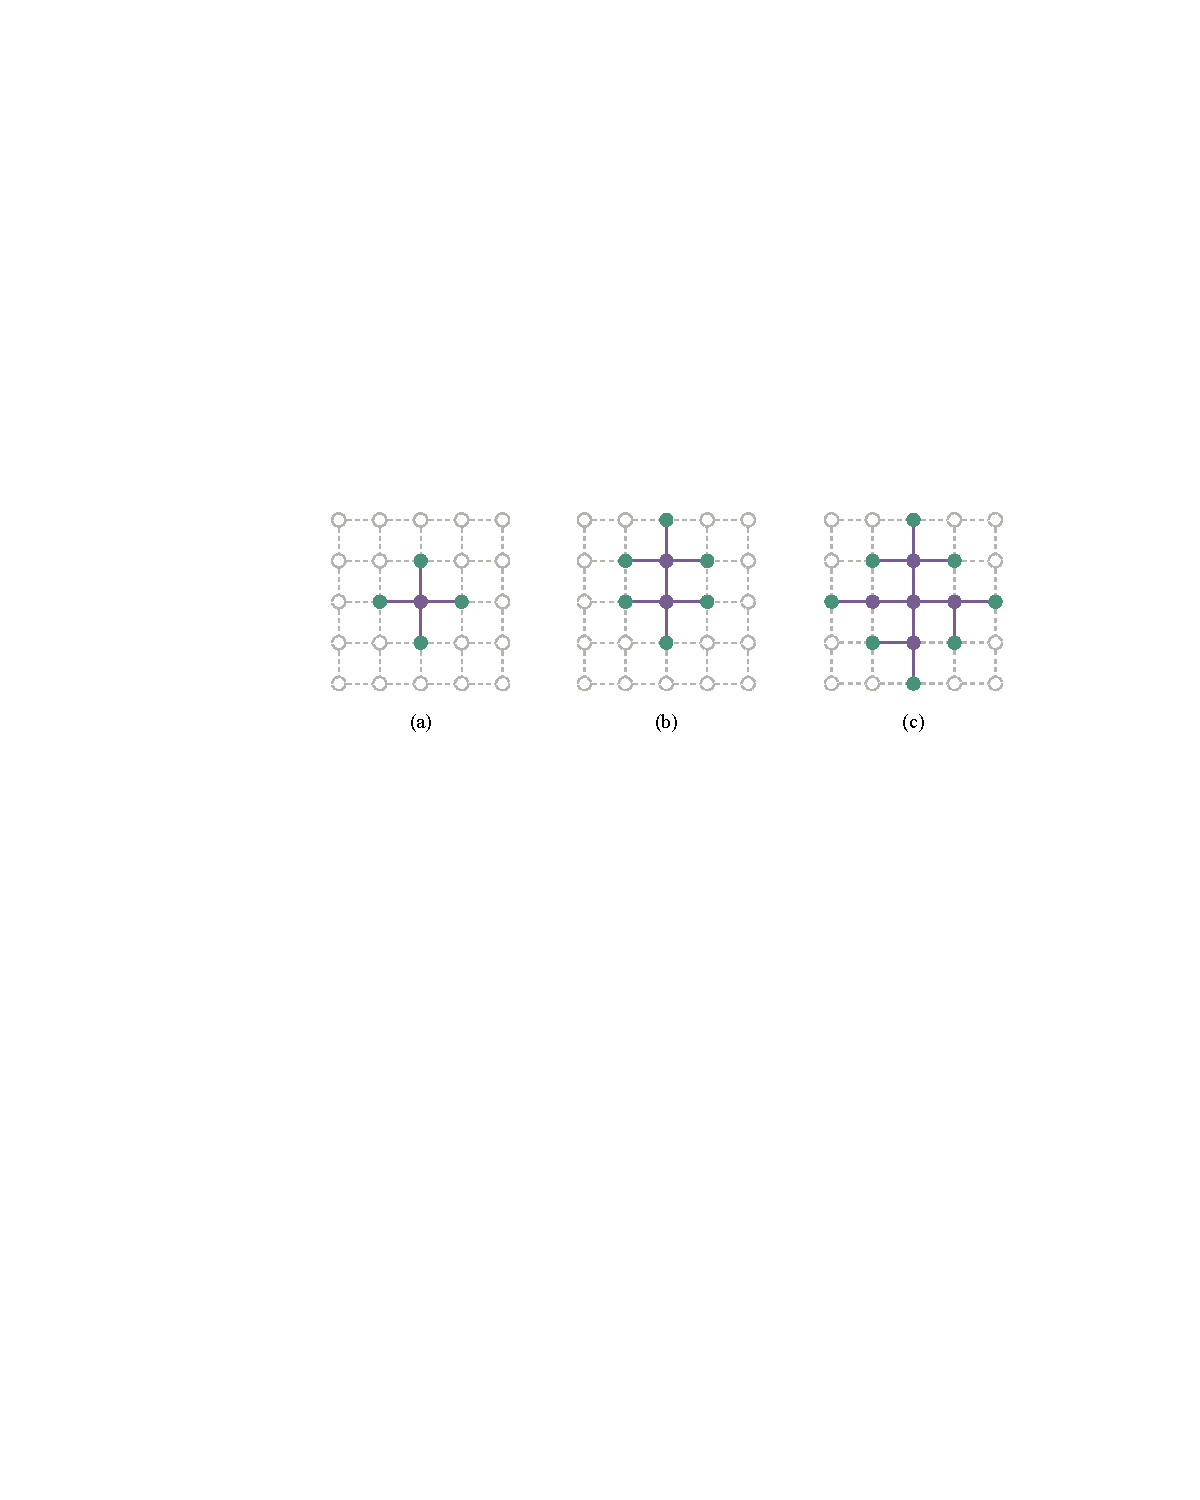
\includegraphics[alt={aima fig 03_06 separation property graph search},width=0.75\linewidth]{aima-fig-03_06-separation-property-graph-search.pdf}


Frontier is in green.  Interior is lavender.  Exterior is faint dashed.

\begin{itemize}
\item (a) Only root expanded.
\item (b) Top frontier node expanded.
\item (c) Remaining successors of root expanded in clockwise order.
\end{itemize}
\section{Redundant Paths}
\label{sec:org934ad77}


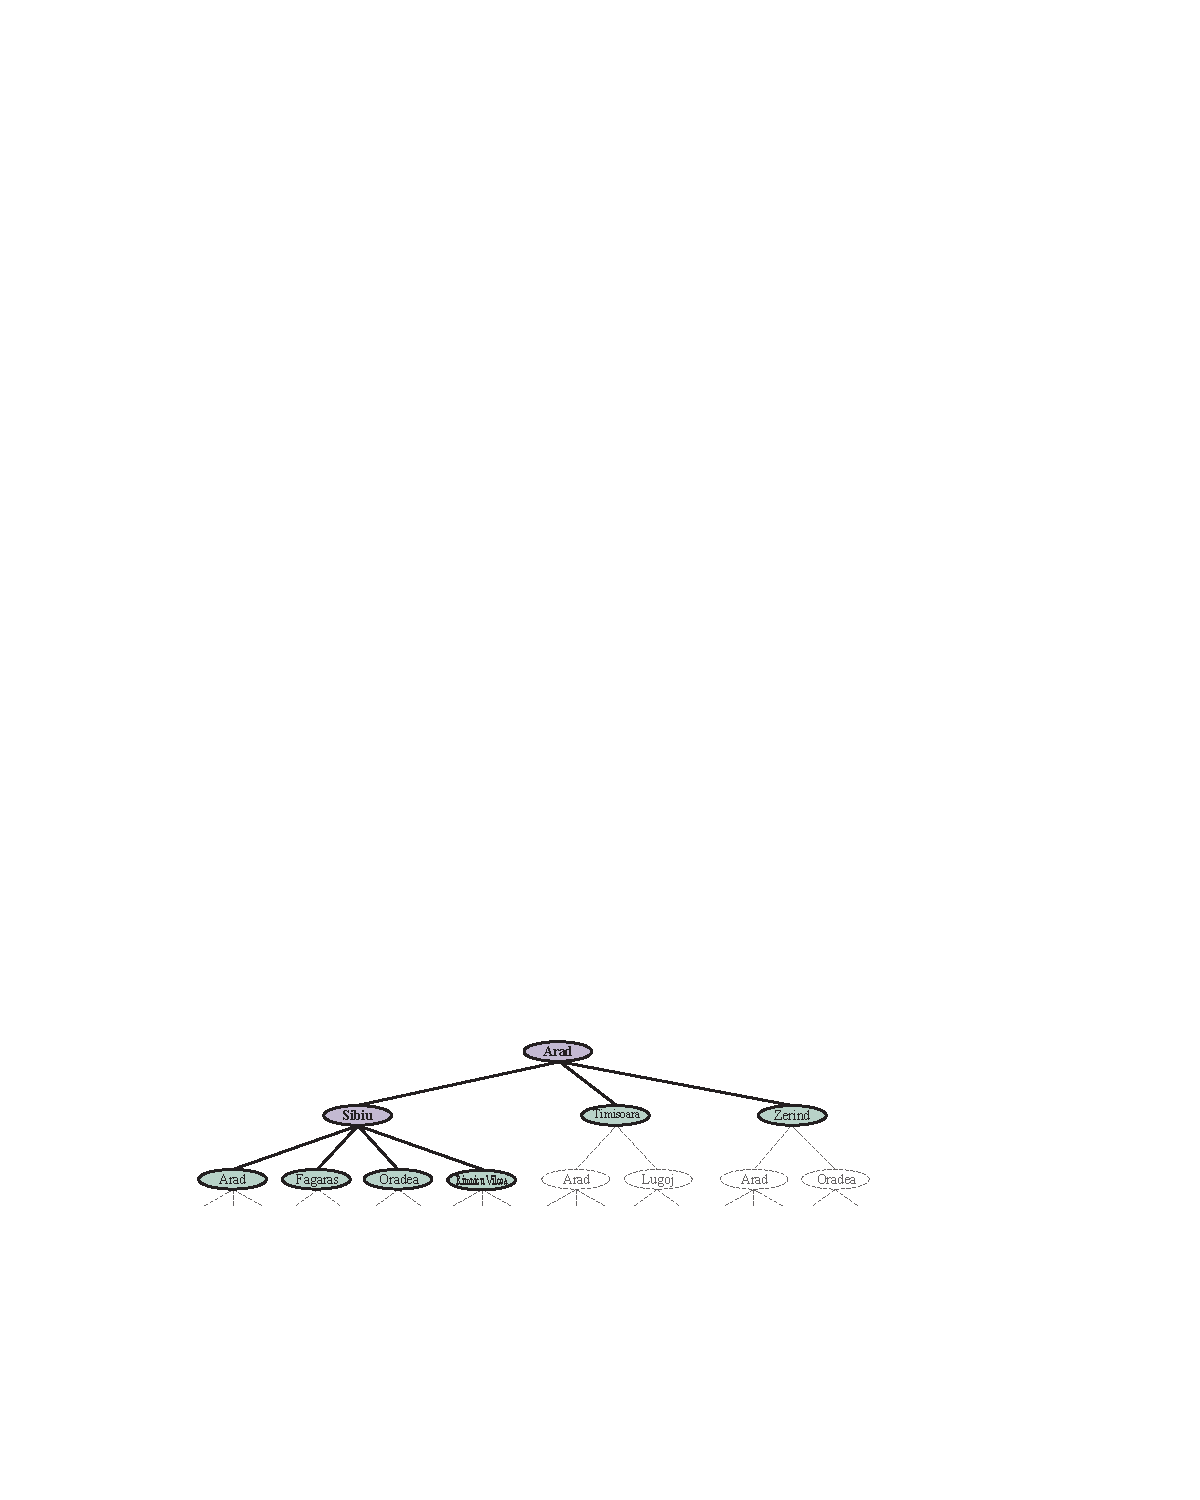
\includegraphics[alt={aima fig 03_04 arad repeated},height=1.2in]{aima-fig-03_04-arad-repeated.pdf}


In the path from \texttt{Arad} to \texttt{Sibiu} to \texttt{Arad},

\begin{itemize}
\item \texttt{Arad} is a \textbf{repeated state} and
\item the path is a \textbf{cycle}, or \textbf{loopy path}.
\end{itemize}

Cycle special case of \textbf{redundant path}: multiple paths to the same state.  Three approaches:

\begin{enumerate}
\item Remember reached states, like best-first search.  Best when reached states fits in memory.
\item Don't worry about repeated states.  Works when repeated states rare or impossible.

\begin{itemize}
\item \textbf{Graph search} checks for redundant paths, which occur in graphs in general.
\item \textbf{Tree-like search} does not check for redundant paths, since trees are acyclic graphs.
\end{itemize}

\item Only check for cycles, not other kinds of redundant paths.

\begin{itemize}
\item E.g., search path in reverse
\end{itemize}
\end{enumerate}
\section{Measuring Problem-Solving Performance}
\label{sec:orgf3ea960}

\begin{itemize}
\item \textbf{Completeness}: Is the algorithm guaranteed to find a solution when there is one, and to correctly report failure when there is not?

\begin{itemize}
\item Complete search algorithms must be \textbf{systematic}.
\item Easier to achieve for finite state spaces.
\item In an infinite state space with no solution, search won't terminate.
\end{itemize}

\item \textbf{Cost optimality}: Does it find a solution with the lowest path cost of all solutions?
\item \textbf{Time complexity}: How long does it take to find a solution? This can be measured in seconds, or more abstractly by the number of states and actions considered.
\item \textbf{Space complexity}: How much memory is needed to perform the search?
\end{itemize}

For \textbf{explicit} graphs, like Romania, time and space complexity typically expressed in terms of number of vertices (state nodes), \(|V|\), and number of edges, \(|E|\) (state-action pairs, which generate (\((s, a, s')\) triples).

For \textbf{implicit} state space graphs we characterize time and space complexity in terms of depth, \(d\) (number of actions in an optimal solution), and branching factor, \(b\) (number of successor nodes per node).  For most of our discussions, we'll use this characterization.
\section{Implementation Note: The \texttt{yield} statement}
\label{sec:orgbe01eab}

A function containing a \texttt{yield} statement is a \textbf{generator}.  Use a generator to turn a data generating process into an iterator.  Node expansion is a data generating process.

\begin{lstlisting}[language=Python,numbers=none]
In [36]: def by_twos(start: int, end: int):
    ...:     x = start
    ...:     while x < end:
    ...:         yield x
    ...:         x += 2
    ...:

In [37]: by_twos(1, 9)
Out[37]: <generator object by_twos at 0x109010ee0>

In [38]: list(Out[37])
Out[38]: [1, 3, 5, 7]

In [39]: for x in by_twos(1, 10):
    ...:     print(f"{x=}")
    ...:
x=1
x=3
x=5
x=7
x=9
\end{lstlisting}
\section{Search Data Structures}
\label{sec:org105587d}

Node:

\begin{itemize}
\item `node.STATE`: the state to which the node corresponds;
\item `node.PARENT`: the node in the tree that generated this node;
\item `node.ACTION`: the action that was applied to the parent’s state to generate this node;
\item `node.PATH-COST`: the total cost of the path from the initial state to this node. In mathematical formulas, we use \(g(node)\) as a synonym for PATH-COST.
\end{itemize}

Frontier is a \textbf{queue} with operations:

\begin{itemize}
\item `IS-EMPTY(frontier)` returns true only if there are no nodes in the frontier.
\item `POP(frontier)` removes the top node from the frontier and returns it.
\item `TOP(frontier)` returns (but does not remove) the top node of the frontier.
\item `ADD(node, frontier)` inserts node into its proper place in the queue.
\end{itemize}

Queues used in search algorithms:

\begin{itemize}
\item A \textbf{priority queue} first pops the node with the minimum cost according to some evaluation function, \(f\) . It is used in best-first search.
\item A \textbf{FIFO queue} or first-in-first-out queue first pops the node that was added to the queue first; we shall see it is used in breadth-first search.
\item A \textbf{LIFO queue} or last-in-first-out queue (also known as a stack) pops first the most recently added node; we shall see it is used in depth-first search.
\end{itemize}
\section{Best-First Search}
\label{sec:org8602b86}

Best-first search is an abstract search algorithm.  Name can be tricky to understand.

\begin{itemize}
\item \textbf{Best} way to pick the \textbf{first} node to consider next.
\item We use a generalization of queues, called a \textbf{priority queue}, to store the \textbf{frontier}.
\item An evaluation function, \(f(node)\), imposes an ordering on the nodes in the priority queue.
\end{itemize}

\begin{quote}
The evaluation function considers the path to the node, not any property of the node itself.  Remember, a solution to a search problem is characterized by the \textbf{path} from the root to the goal, not some characteristic of the goal.
\end{quote}
\section{Best-First Search Algorithm}
\label{sec:org4870f25}


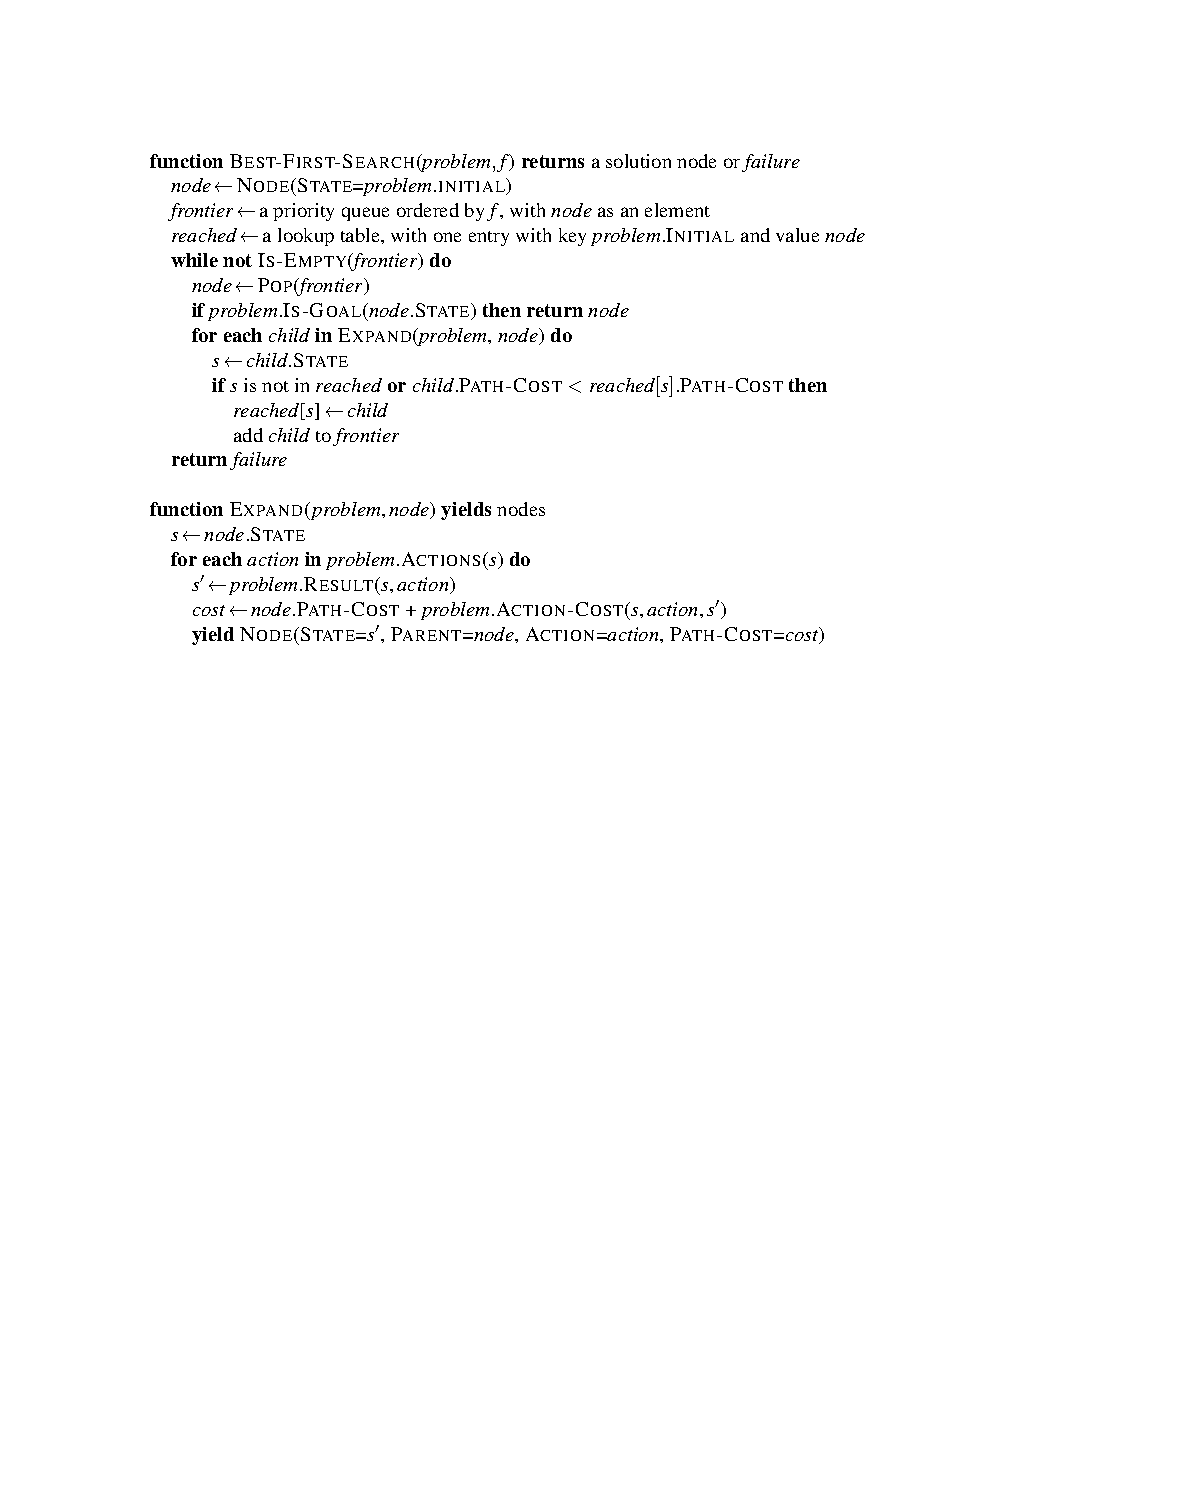
\includegraphics[alt={aima fig 03_07 best first search algorithm},height=3.2in]{aima-fig-03_07-best-first-search-algorithm.pdf}


We'll now describe several uninformed search algorithms.  I recommend you also look at their \href{https://github.com/aimacode/aima-python/blob/master/search4e.ipynb}{implementations in Python}, which may be easier to follow.
\section{Uninformed Search Strategies}
\label{sec:orgf20bcfd}

Uninformed search strategies have no information about which actions are better for reaching a goal.  In these cases we can only do systematic searches of the state space.  We'll discuss

\begin{itemize}
\item Breadth-first search
\item Uniform-Cost search (Djikstra's algorithm)
\item Depth-first search
\item Depth-limited searchand
\item Iterative deepening search.
\item Bidirectional search
\end{itemize}
\section{Breadth-First Search}
\label{sec:orgad994dd}

\begin{itemize}
\item Good when path costs are uniform.
\item Equivalent to best-first search where \(f(node)\) is the depth of the node
\item Guaranteed to find minimal number of actions because it evaluates depth \(d\) before generating depth \(d+1\).
\end{itemize}

But three optimizations afforded by the BFS algorithm and uniform path costs:

\begin{itemize}
\item FIFO queue instead of priority queue
\item \textbf{Reached} is a set instead of a mapping \(S \rightarrow Node\)

\begin{itemize}
\item With uniform path costs, as soon as BFS finds a node, it's the fastest way to it.
\end{itemize}

\item \textbf{Early goal test} -- as soon as we expand a node, we can test it.
\end{itemize}
\section{BFS Algorithm}
\label{sec:orgb2f7220}


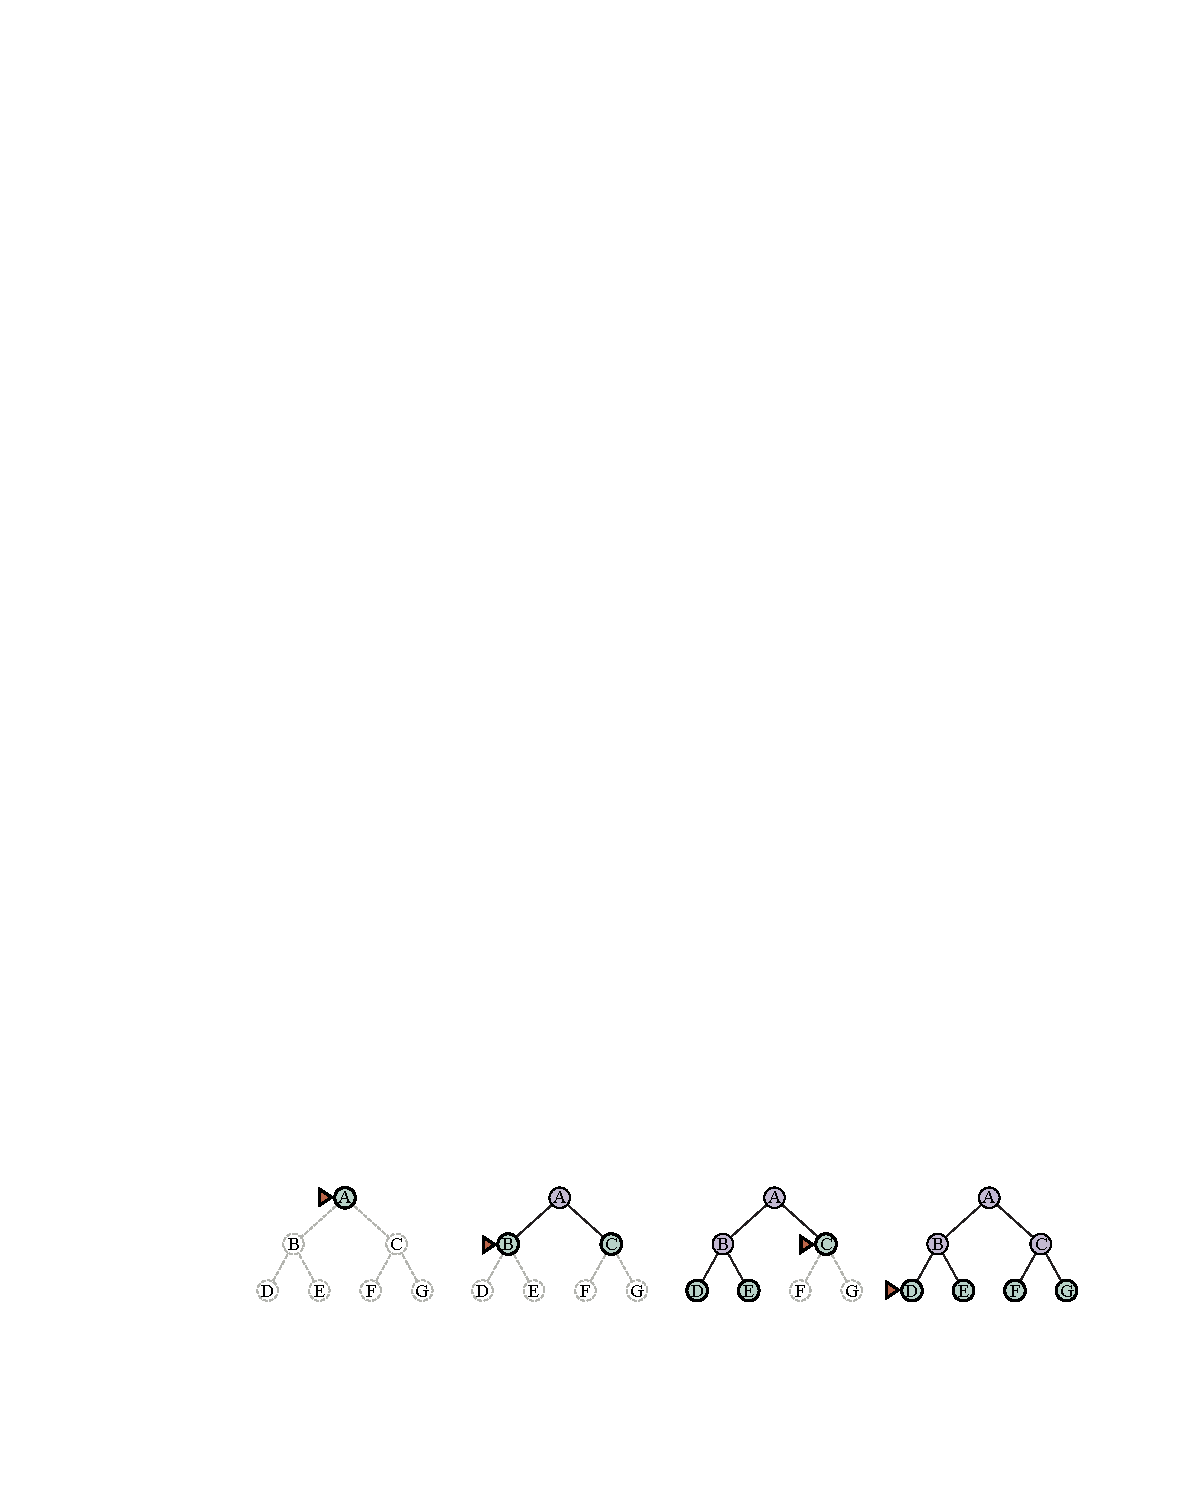
\includegraphics[alt={aima fig 03_08 bfs binary tree},height=0.8in]{aima-fig-03_08-bfs-binary-tree.pdf}



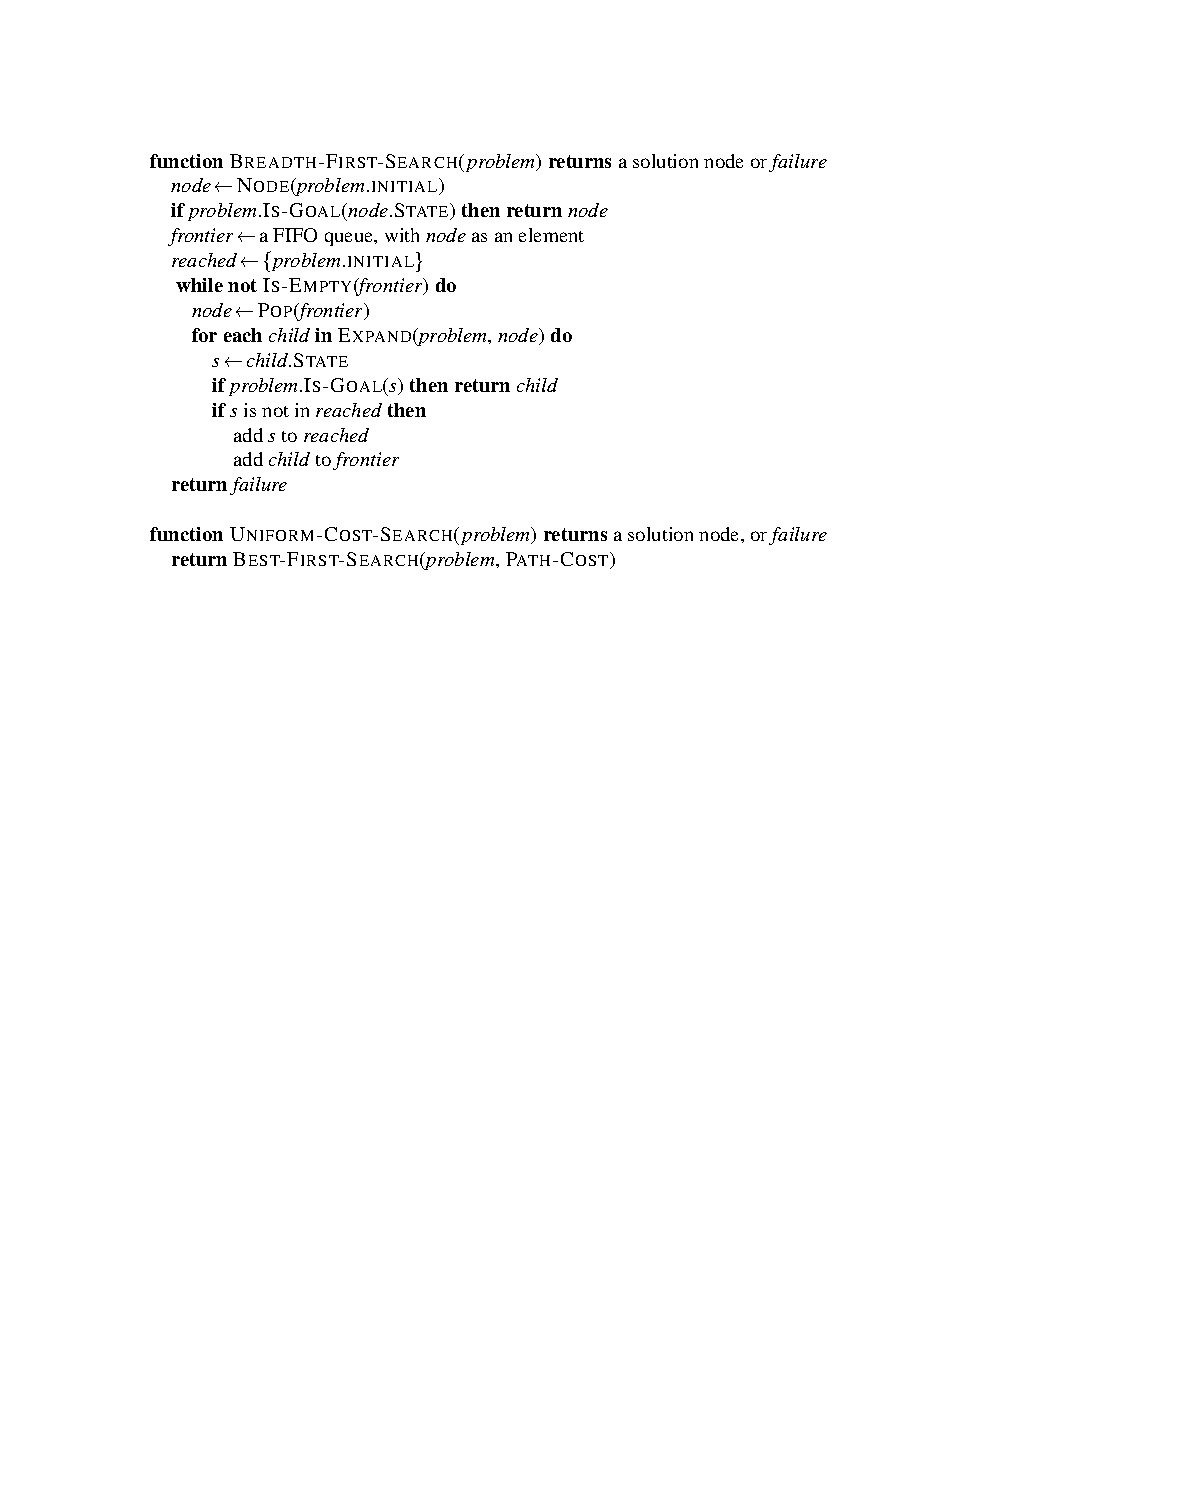
\includegraphics[alt={aima fig 03_09 bfs algorithm},height=2.4in]{aima-fig-03_09-bfs-algorithm.pdf}
\section{Analysis of BFS}
\label{sec:org28062d1}

\begin{itemize}
\item Complete, because it generates all nodes at each depth.
\item Time complexity: at each level, \(b\) nodes for  each \(b\) predecessors, so

\begin{itemize}
\item \(1 + b + b^2 + b^3 + \cdots + b^d = O(b^d)\)
\end{itemize}

\item Space complexity: \(O(b^d)\) because all nodes are stored while the search proceeds.
\end{itemize}

Uninformed search is not appropriate for exponential complexity problems except for smallest instances.  Assuming your computer can process 1 million nodes per second and store each node in 1 Kb,

\begin{itemize}
\item For a problem with \(b = 10\) and \(d = 10\), how long will it take search and how much space will be required?
\item Same problem, but with \(d = 14\)?
\end{itemize}
\section{Uniform-Cost Search (Dijkstra's Algorithm)}
\label{sec:org2d882ab}

BFS where the best-first \(f(node)\) is the path cost to the current node.


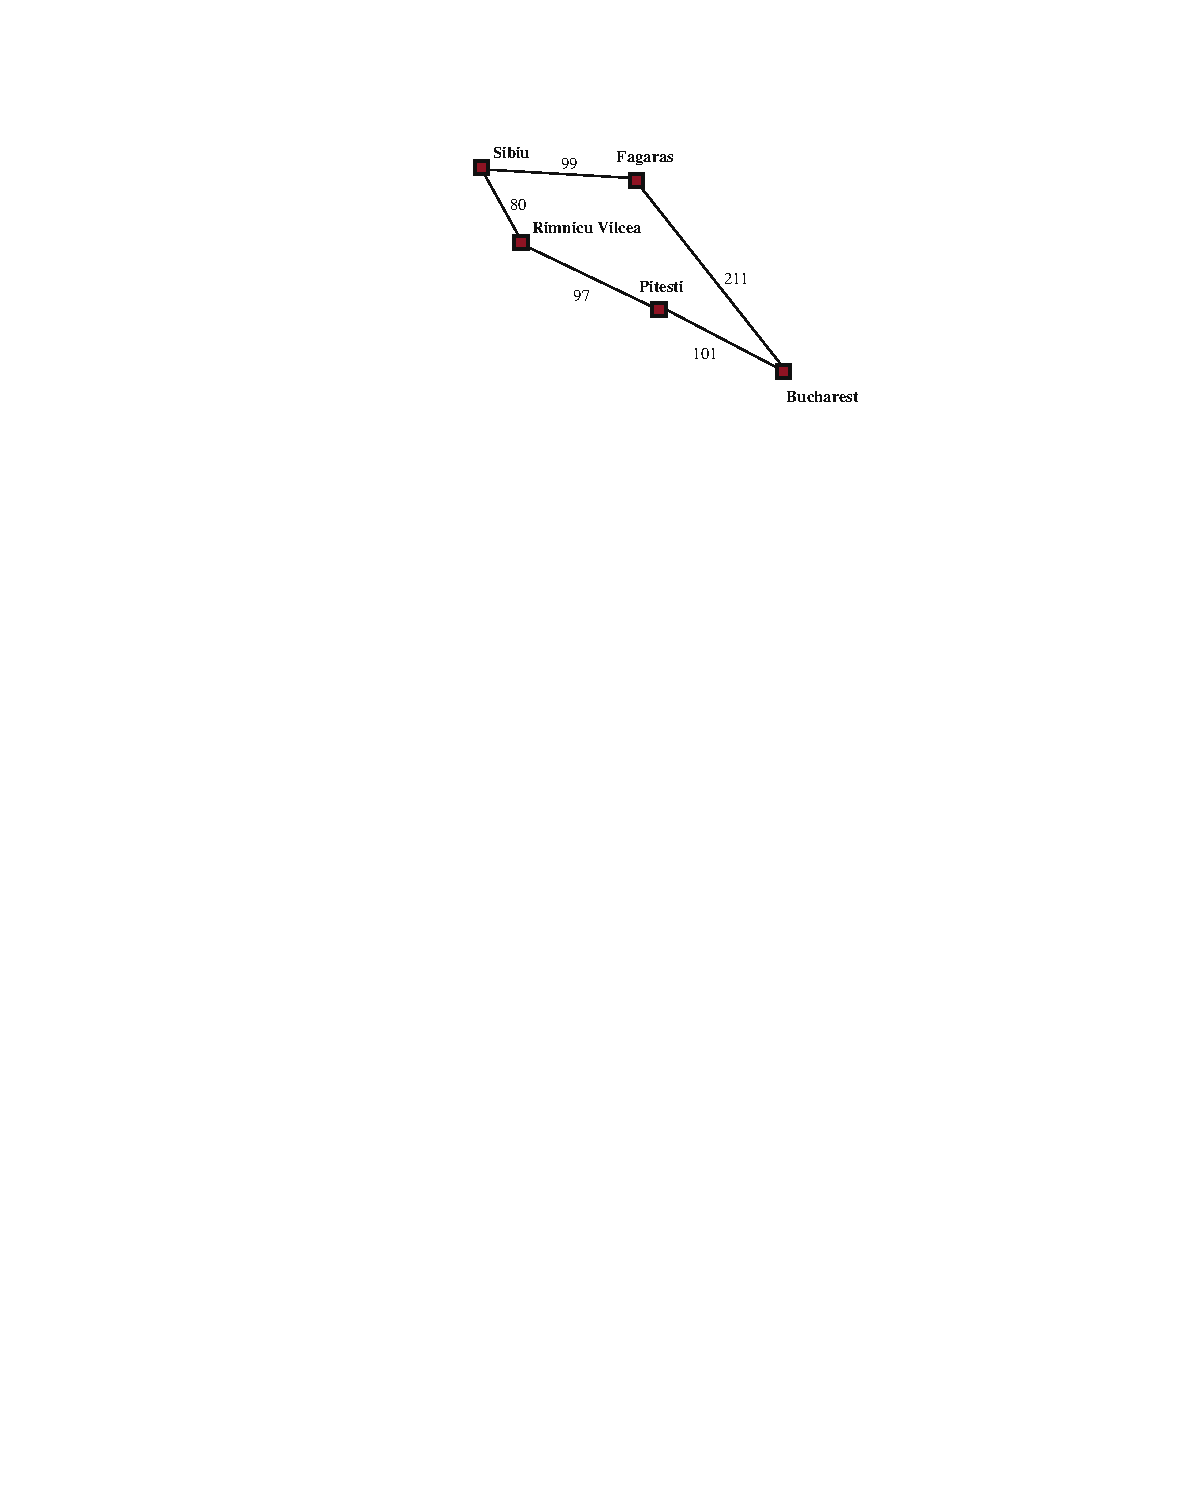
\includegraphics[alt={aima fig 03_10 sibiu bucharest},height=1.2in]{aima-fig-03_10-sibiu-bucharest.pdf}


\begin{itemize}
\item From Sibiu, exand Faragas and RV.
\item Path cost to RV is less, so it's expanded next, adding Pitesti to frontier.
\item Path cost to Pitesti is 80 + 97 = 177, so Faragas is expanded next, adding Bucharest, the goal to the frontier with a total path cost of 99 + 211 = 310.

\begin{itemize}
\item Goal test not applied to a node until it's expanded, so \ldots{}
\end{itemize}

\item Expand Pitesti, which adds Bucharest, the goal, to the frontier with a path cost of 177 + 101 = 278

\begin{itemize}
\item 278 < 310, so this is not at head of priority queue.
\end{itemize}

\item Apply goal test to Bucharest node before expansion, finding it to be the goal.
\end{itemize}
\section{Analysis of Uniform-Cost Search}
\label{sec:orgc71be30}

Let \(C^*\) be the cost of the optimal solution and \(\epsilon > 0\) be a lower bound on the cost of each action.


\begin{itemize}
\item Complete, like BFS
\item Cost-optimal, because a solution will be at least as low cost as any other in the frontier.
\item Time and space complexity are \(O(b^{1 + \lfloor \frac{C^*}{\epsilon} \rfloor})\).

\begin{itemize}
\item Since lower cost paths are always explored first, even when a higher cost path might be the one to lead to an optimal solution, can be worse than BFS.
\item If all action costs equal, then it's like BFS, \(O(b^{1 + d})\).
\end{itemize}
\end{itemize}
\section{Depth-First Search - FIFO Frontier}
\label{sec:org05ff64e}


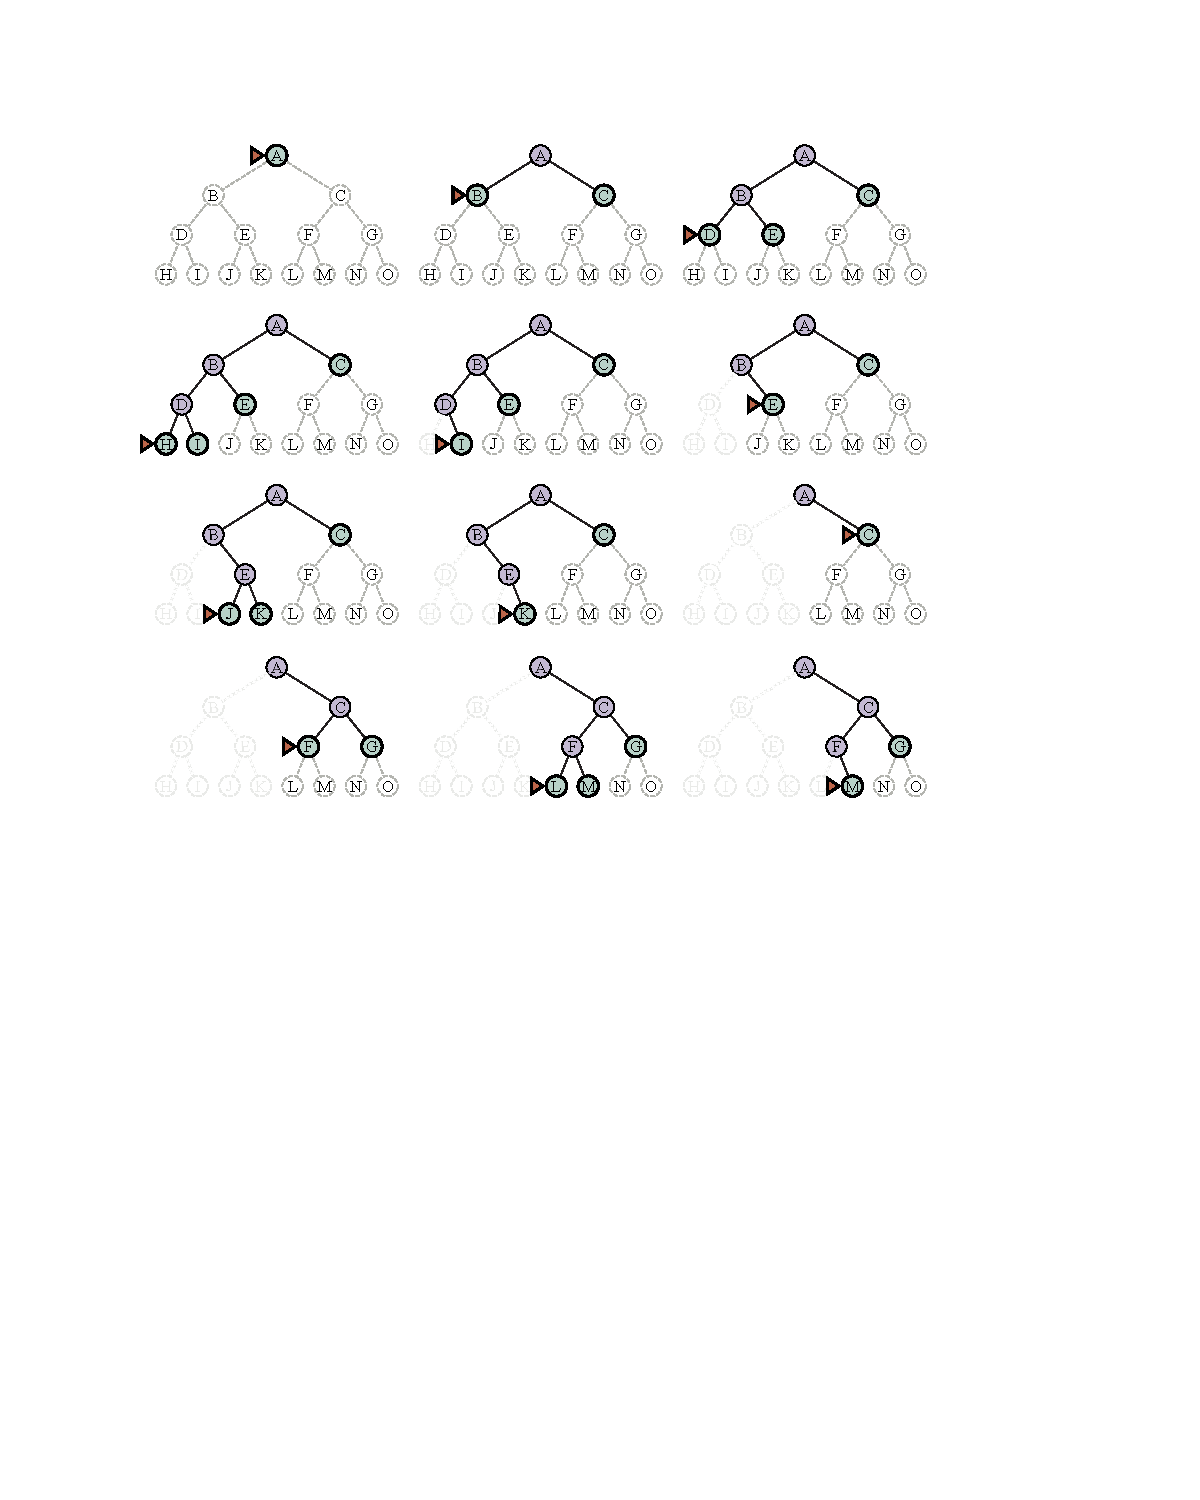
\includegraphics[alt={aima fig 03_11 dfs progress},height=3.6in]{aima-fig-03_11-dfs-progress.pdf}
\section{Analysis of DFS}
\label{sec:orgbb6c67e}

\begin{itemize}
\item Not cost-optimal -- returns first solution it finds
\item For state space that are finite trees:

\begin{itemize}
\item Complete
\item Time \(O(n)\) where \(n\) is number of states
\item Space: \(O(bm)\), where \(b\) is branching factor and \(m\) is max depth of tree.
\end{itemize}

\item For (acyclic) graph state spaces, may expand same state via multiple paths.

\begin{itemize}
\item For cyclic graph state spaces, need to check for cycles to prevent infinite loops.
\end{itemize}

\item For infinite state spaces, not complete -- may get stuck in an infinite subtree.
\end{itemize}

Why bother with DFS at all? \textbf{Memory efficiency}
\section{Depth-Limited Search}
\label{sec:org3725f65}


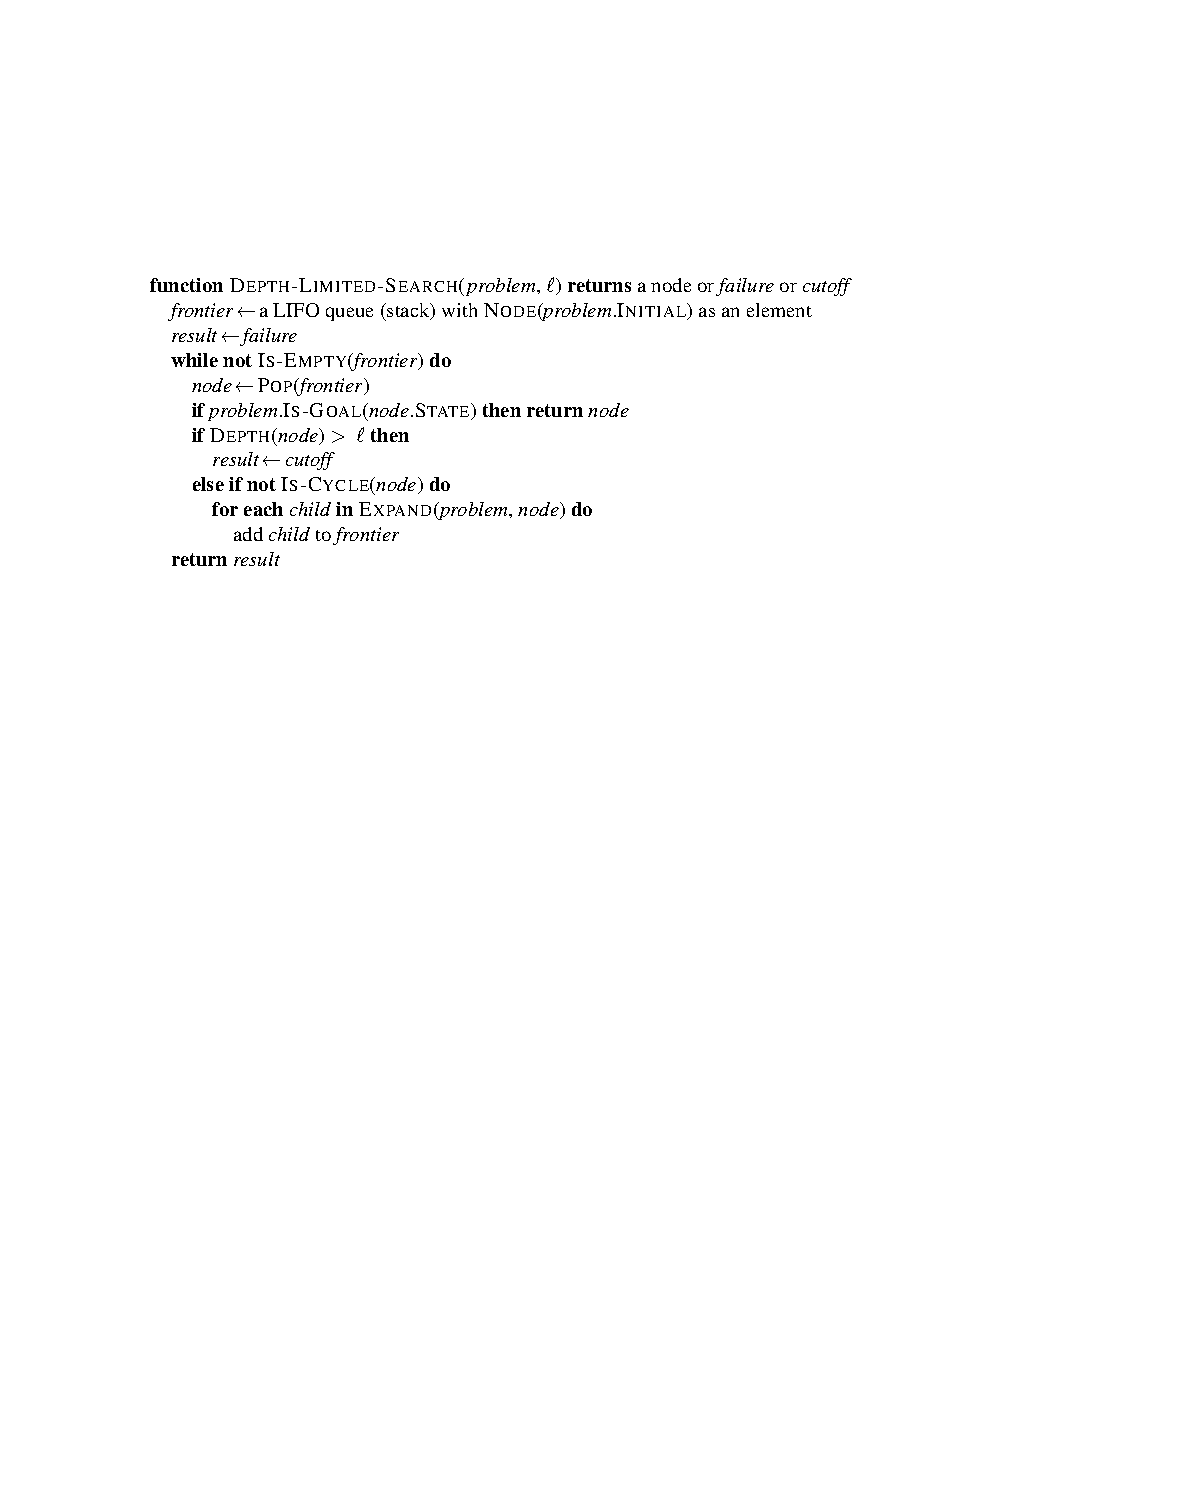
\includegraphics[alt={aima fig 03_12 depth limited search algorithm},width=0.75\linewidth]{aima-fig-03_12-depth-limited-search-algorithm.pdf}


\begin{itemize}
\item If limit, \(\ell\), too small, won't find goal.
\item To guarantee completeness, choose \(\ell \ge diameter\)

\begin{itemize}
\item Diameter of a state space graph: maximum number of actions necessary to transition from any state to any other state.
\end{itemize}
\end{itemize}
\section{Iterative Deepening Search}
\label{sec:orge691bb4}


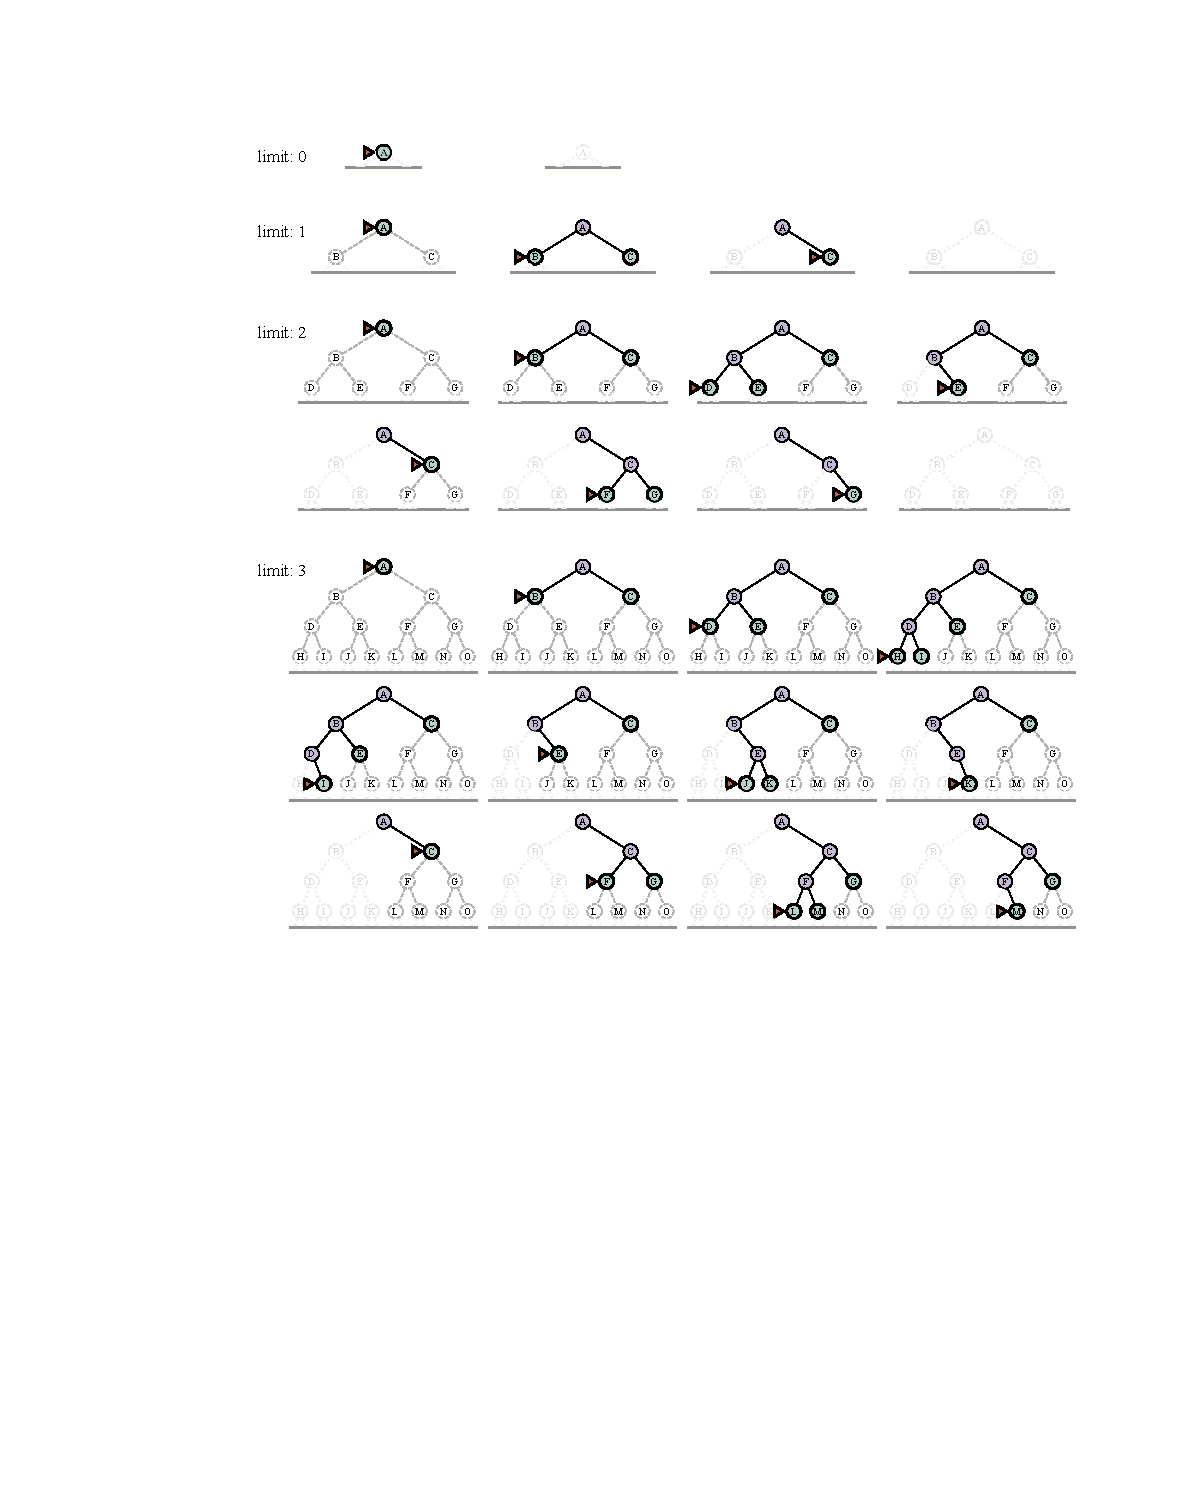
\includegraphics[alt={aima fig 03_13 iterative deepening progress},height=3.6in]{aima-fig-03_13-iterative-deepening-progress.pdf}
\section{Analysis of Iterative Deepening Search}
\label{sec:orga877902}

\begin{itemize}
\item Cost-optimal for state spaces where all actions have same cost.
\item For state space that are finite trees, where \(b\) is branching factor and \(m\) is max depth of tree:

\begin{itemize}
\item Complete for finite acyclic spaces, or finite cyclic spaces with cycle checking
\item Space: \(O(bd)\) if there is a solution, \(O(bm)\) if no solution,
\item Time \(O(b^d)\) if there is a solution, \(O(b^m)\) if no solution.

\begin{itemize}
\item \(N(IDS) = (d)b^1 + (d-1)b^2 + \cdots + b^d\)
\end{itemize}
\end{itemize}
\end{itemize}


\begin{itemize}
\item For (acyclic) graph state spaces, may expand same state via multiple paths.

\begin{itemize}
\item For cyclic graph state spaces, need to check for cycles to prevent infinite loops.
\end{itemize}

\item For infinite state spaces, not complete -- may get stuck in an infinite subtree.
\end{itemize}

\begin{quote}
In general, iterative deepening search is the preferred uninformed search method when the search state space is larger than can fit in memory and The depth of the solution is not known.
\end{quote}
\section{Bidirectional Best-First Search}
\label{sec:org26c342f}


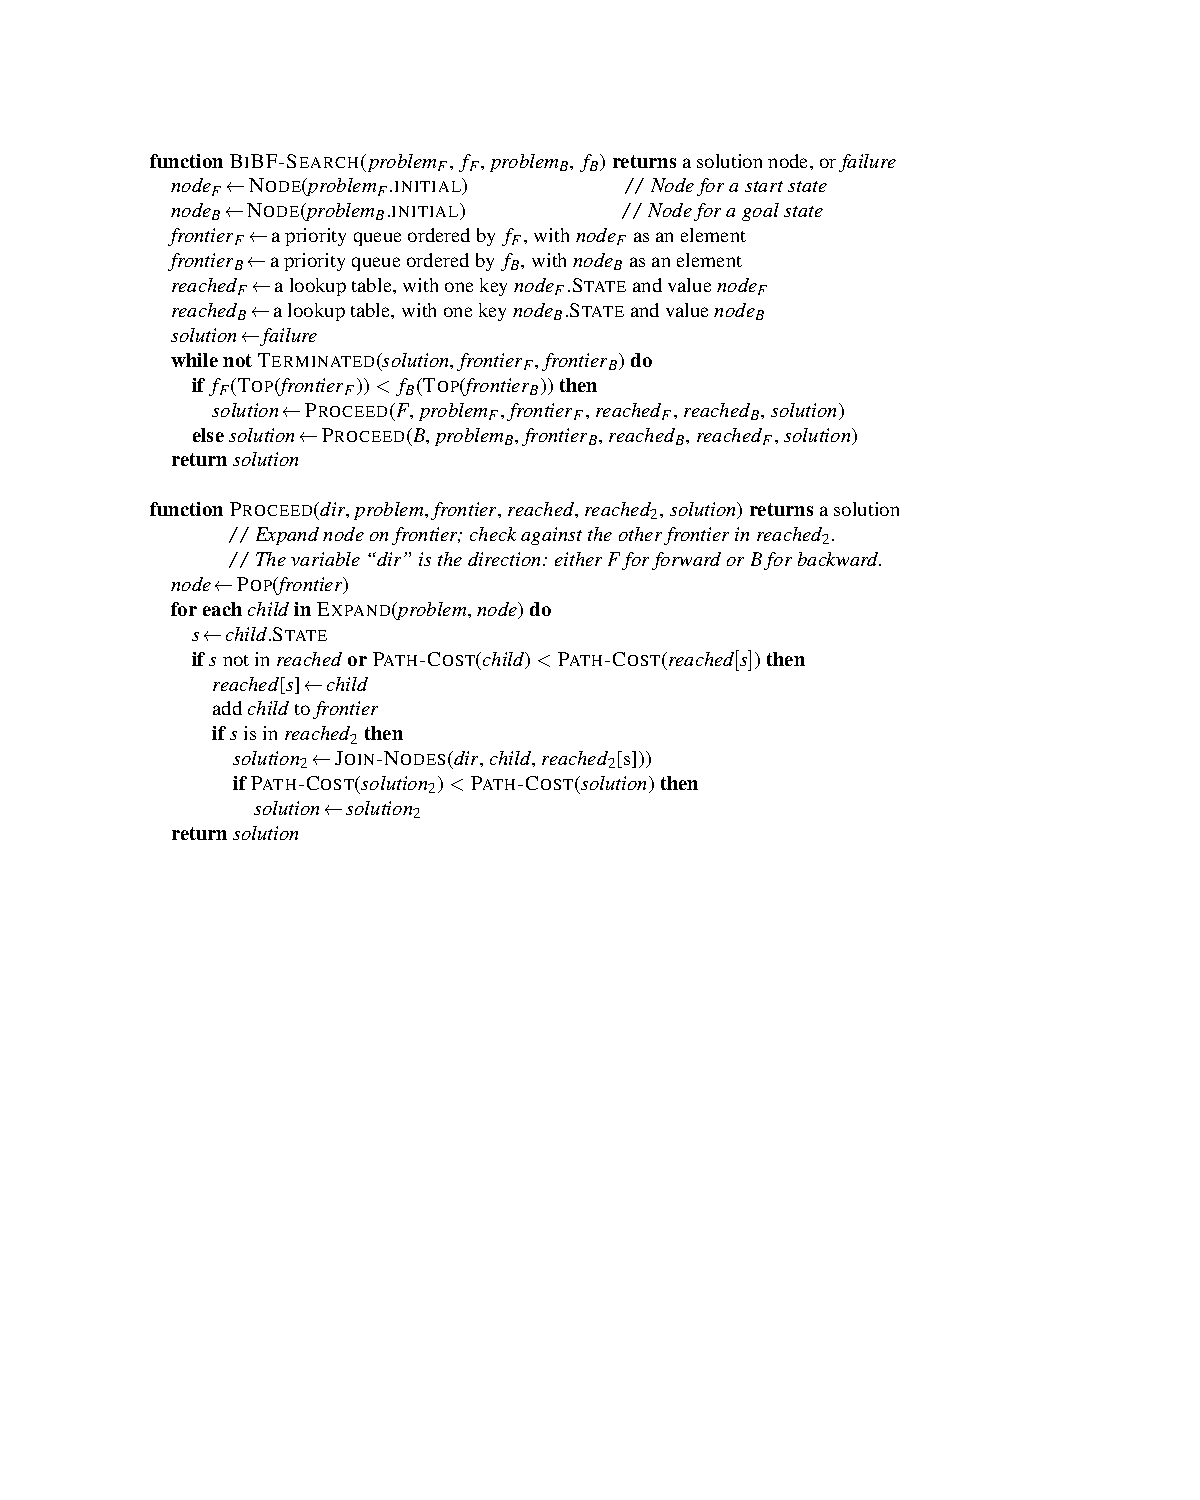
\includegraphics[alt={aima fig 03_14 bidirectional best first search algorithm},height=3.2in]{aima-fig-03_14-bidirectional-best-first-search-algorithm.pdf}


Motivation: \(b^{\frac{d}{2}} + b^{\frac{d}{2}} \ll b^d\).
\section{Comparing Uninformed Search Algorithms}
\label{sec:orgf40b539}


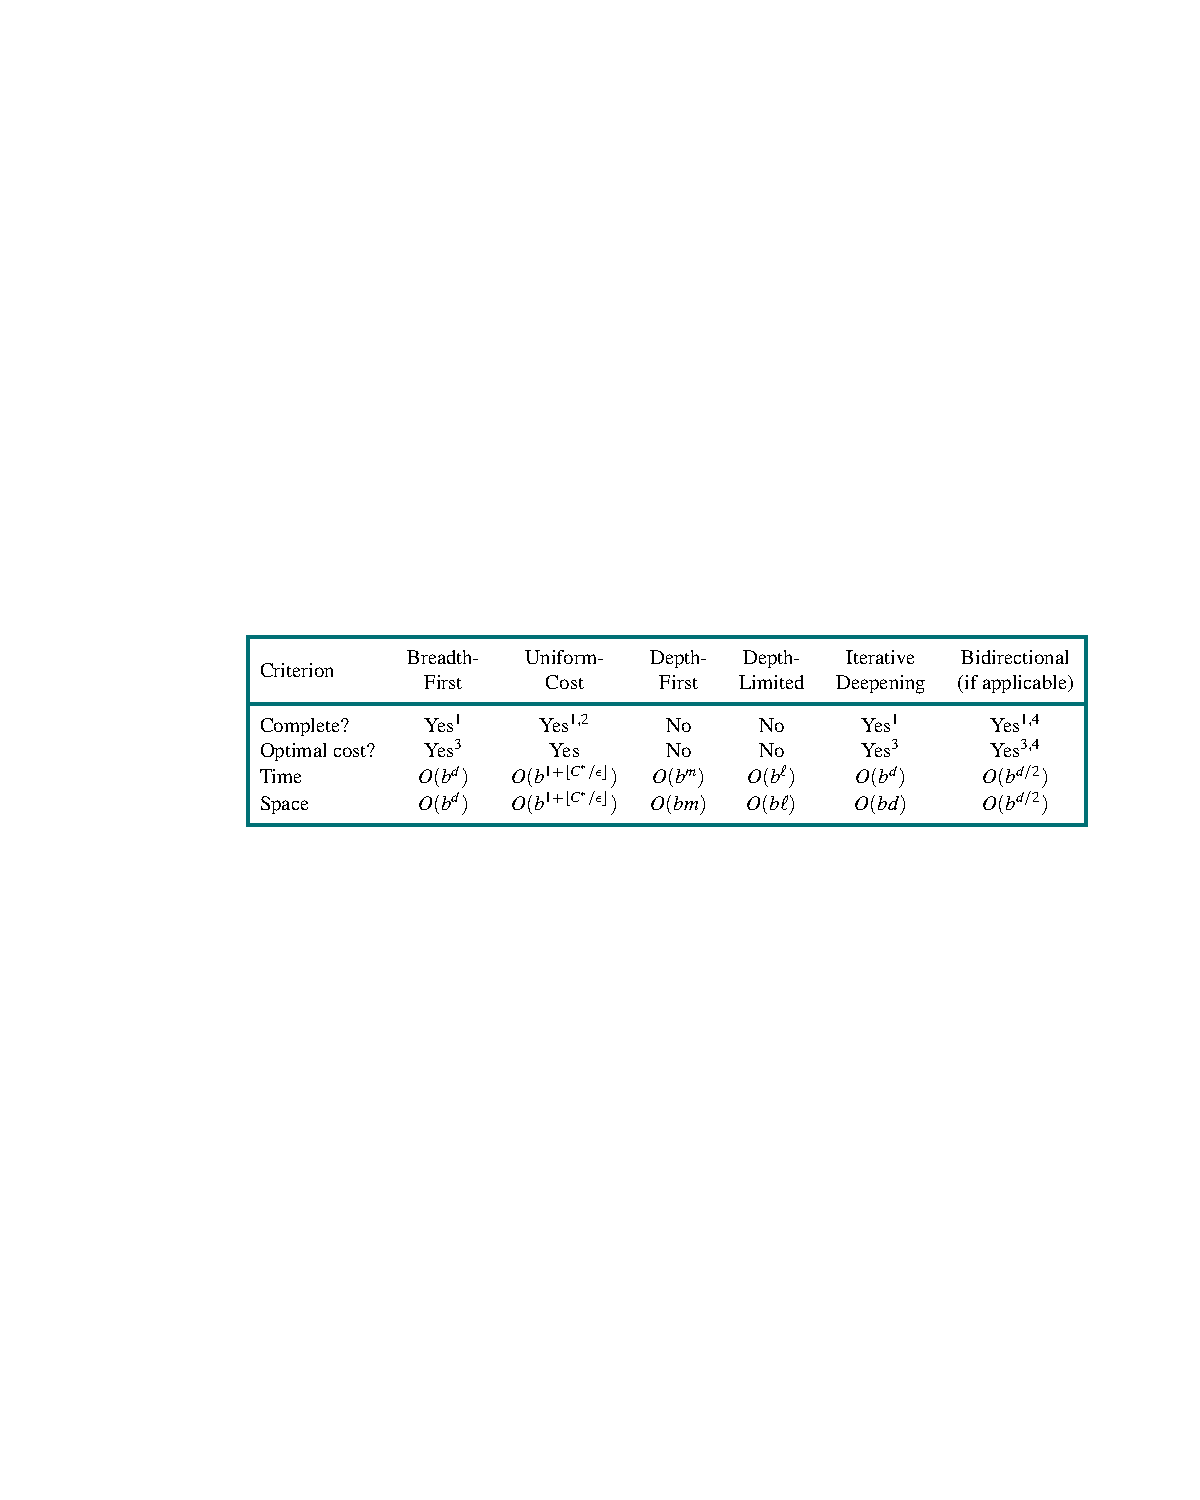
\includegraphics[alt={aima fig 03_15 uninformed search comparisons},width=0.75\linewidth]{aima-fig-03_15-uninformed-search-comparisons.pdf}


Notes:

\begin{itemize}
\item 1: complete if \(b\) is finite, and the state space either has a solution or is finite
\item 2: complete if all action costs are \(\ge \epsilon > 0\)
\item 3: cost-optimal if action costs are all identical
\item 4: if both directions are breadth-first or uniform-cost
\end{itemize}
\end{document}
